\documentclass[12pt,a4paper]{article}
\usepackage[a4paper, margin=0.8in, headheight=14pt]{geometry}
\usepackage{fontspec}
\usepackage{unicode-math}
\setmainfont{TeX Gyre Pagella}
\setmonofont[Scale=0.88]{TeX Gyre Cursor}
\setmathfont{Latin Modern Math}
\usepackage{xcolor}
\usepackage{colortbl}
\usepackage{titlesec}
\usepackage{enumitem}
\usepackage{tabularx}
\usepackage{booktabs}
\usepackage{array}
\usepackage{amsmath}
\usepackage{tikz}
\usetikzlibrary{shapes.geometric, arrows.meta, positioning, calc, fit, decorations.pathreplacing, decorations.pathmorphing, patterns}
\usepackage[american]{circuitikz}
\usepackage{tcolorbox}
\tcbuselibrary{skins, breakable}
\usepackage{hyperref}
\usepackage{fancyhdr}
\usepackage{graphicx}
\usepackage{microtype}
\hyphenpenalty=10000
\exhyphenpenalty=10000
\sloppy
\usepackage{caption}
\usepackage{setspace}
\usepackage{multirow}
\usepackage{tocloft}
\newcommand{\Q}[1]{\textbf{#1}\par\noindent\ignorespaces}
\definecolor{myred}{RGB}{196,30,58}
\definecolor{mydark}{RGB}{30,30,50}
\definecolor{mygreen}{RGB}{14,120,80}
\definecolor{myteal}{RGB}{0,130,140}
\definecolor{myamber}{RGB}{180,100,0}
\definecolor{mypurple}{RGB}{100,30,160}
\definecolor{mygray}{RGB}{246,247,249}
\definecolor{mgframe}{RGB}{180,185,200}
\definecolor{watermark}{RGB}{145,150,170}
\definecolor{hdrred}{RGB}{250,232,235}
\definecolor{hdrgreen}{RGB}{220,244,233}
\definecolor{hdrteal}{RGB}{220,242,244}
\definecolor{hdramber}{RGB}{253,242,215}
\definecolor{hdrpurple}{RGB}{238,228,255}
\definecolor{hdrgray}{RGB}{238,240,245}
\definecolor{rowalt}{RGB}{250,251,253}

\titleformat{\section}{\large\bfseries\color{myred}}{\thesection.}{0.5em}{}[\vspace{1pt}{\color{myred}\rule{\linewidth}{0.8pt}}]
\titleformat{\subsection}{\normalsize\bfseries\color{myteal}}{\thesubsection}{0.5em}{}
\titlespacing*{\section}{0pt}{18pt}{7pt}
\titlespacing*{\subsection}{0pt}{11pt}{4pt}
\setlength{\parindent}{0pt}
\setlength{\parskip}{4pt}
\renewcommand{\cfttoctitlefont}{\large\bfseries\color{myred}}
\renewcommand{\cftaftertoctitle}{\par\noindent{\color{myred}\rule{\linewidth}{0.8pt}}}
\setlength{\cftbeforetoctitleskip}{0pt}
\setlength{\cftaftertoctitleskip}{6pt}
\renewcommand{\cftsecfont}{\normalsize\bfseries\color{mydark}}
\renewcommand{\cftsecpagefont}{\normalsize\bfseries\color{mydark}}
\renewcommand{\cftsecleader}{\cftdotfill{\cftdotsep}}
\setlength{\cftbeforesecskip}{7pt}
\renewcommand{\cftsubsecfont}{\small\color{mydark}}
\renewcommand{\cftsubsecpagefont}{\small\color{mydark}}
\setlength{\cftbeforesubsecskip}{3pt}
\setlength{\cftsubsecindent}{1.4em}
\renewcommand{\cftpartfont}{\normalsize\bfseries\color{myteal}}
\renewcommand{\cftpartpagefont}{\normalsize\bfseries\color{myteal}}
\setlength{\cftbeforepartskip}{14pt}
\renewcommand{\arraystretch}{1.45}
\setlength{\tabcolsep}{6pt}
\arrayrulecolor{mydark}
\newcolumntype{B}[1]{>{\small\bfseries\raggedright\arraybackslash}m{#1}}
\newcolumntype{C}[1]{>{\centering\arraybackslash}m{#1}}
\newcolumntype{Y}{>{\small\raggedright\arraybackslash}X}
\renewcommand{\tabularxcolumn}[1]{m{#1}}
\newcommand{\currmodule}{Module 1}
\pagestyle{fancy}
\fancyhf{}
\fancyhead[L]{\small\color{myred}\textbf{PE-EC603A}\;\color{mydark}--- Introduction to MEMS}
\fancyhead[R]{\small\color{myteal}\textbf{\currmodule\ Notes}}
\fancyfoot[C]{\small\color{mydark}\thepage}
\fancyfoot[R]{\small\color{watermark}\textit{\copyright\ Biraj}}
\renewcommand{\headrulewidth}{0.5pt}
\renewcommand{\footrulewidth}{0.3pt}

\hypersetup{colorlinks=true, linkcolor=myteal, urlcolor=myteal,
  pdfauthor={Biraj Sarkar},
  pdftitle={PE-EC603A --- Combined Notes}}

\tcbset{
  tikzbox/.style={
    colback=mygray, colframe=mgframe, boxrule=0.6pt, arc=4pt,
    left=8pt, right=8pt, top=6pt, bottom=6pt,
    colbacktitle=mgframe, coltitle=mydark,
    fonttitle=\small\bfseries
  },
  defbox/.style={
    colback=hdrgreen, colframe=mygreen, boxrule=0.8pt, arc=4pt,
    left=9pt, right=9pt, top=6pt, bottom=6pt,
    colbacktitle=mygreen, coltitle=white,
    fonttitle=\small\bfseries
  },
  formulabox/.style={
    colback=hdrteal, colframe=myteal, boxrule=0.8pt, arc=4pt,
    left=9pt, right=9pt, top=7pt, bottom=7pt,
    colbacktitle=myteal, coltitle=white,
    fonttitle=\small\bfseries
  },
  examplebox/.style={
    colback=hdramber, colframe=myamber, boxrule=0.8pt, arc=4pt,
    left=9pt, right=9pt, top=6pt, bottom=6pt,
    colbacktitle=myamber, coltitle=white,
    fonttitle=\small\bfseries
  },
  masonbox/.style={
    colback=hdrpurple, colframe=mypurple, boxrule=0.8pt, arc=4pt,
    left=9pt, right=9pt, top=6pt, bottom=6pt,
    colbacktitle=mypurple, coltitle=white,
    fonttitle=\small\bfseries
  },
  exambox/.style={
    colback=hdrpurple, colframe=mypurple, boxrule=1pt, arc=5pt,
    left=10pt, right=10pt, top=8pt, bottom=8pt,
    colbacktitle=mypurple, coltitle=white,
    fonttitle=\bfseries,
    breakable, title after break={\textbf{Frequently Asked / Viva Questions (contd.)}}}
}
\tcbset{breakable}
\tcbset{after={\color{black}}}

\tikzset{
  block/.style={rectangle, draw=myteal, fill=hdrteal,
    text width=2.4cm, align=center, minimum height=0.95cm,
    font=\small, rounded corners=3pt, line width=0.7pt},
  redblock/.style={rectangle, draw=myred, fill=hdrred,
    text width=2.4cm, align=center, minimum height=0.95cm,
    font=\small, rounded corners=3pt, line width=0.7pt},
  netnode/.style={rectangle, draw=myteal, fill=hdrteal,
    text width=1.5cm, align=center, minimum height=0.8cm,
    font=\small, rounded corners=3pt, line width=0.7pt},
  sumjunc/.style={circle, draw=myamber, fill=hdramber,
    minimum size=0.62cm, font=\small, line width=0.8pt},
  snode/.style={circle, draw=mypurple, fill=hdrpurple,
    minimum size=0.55cm, font=\footnotesize, line width=0.7pt},
  arrow/.style={-Stealth, thick, color=mydark},
  redarrow/.style={-Stealth, thick, color=myred},
  line/.style={thick, color=mydark}
}

\newcommand{\modulestart}[2]{%
  \clearpage
  \renewcommand{\currmodule}{Module #1}%
  \renewcommand{\theHsection}{mod#1.\arabic{section}}%
  \renewcommand{\theHsubsection}{\theHsection.\arabic{subsection}}%
  \renewcommand{\theHsubsubsection}{\theHsubsection.\arabic{subsubsection}}%
  \phantomsection
  \addcontentsline{toc}{part}{Module #1: #2}%
  \setcounter{section}{0}%
  \begin{center}
    \vspace*{1.0cm}
    {\Huge\bfseries\color{myred} Module #1}\\[10pt]
    {\Large\bfseries\color{mydark} #2}\\[10pt]
    {\color{myred}\rule{0.55\linewidth}{1.2pt}}
  \end{center}
  \vspace{14pt}
}
\begin{document}

\thispagestyle{empty}

% ─── Page Border (TikZ Overlay) ────────────────────────────────────────────────
\begin{tikzpicture}[remember picture, overlay]
  % Outer border (fine line in mgframe)
  \draw[color=mgframe, line width=1.5pt] 
    ($(current page.north west) + (0.6in, -0.6in)$) rectangle 
    ($(current page.south east) + (-0.6in, 0.6in)$);
  % Inner border (finer accent line in myred)
  \draw[color=myred, line width=0.8pt] 
    ($(current page.north west) + (0.65in, -0.65in)$) rectangle 
    ($(current page.south east) + (-0.65in, 0.65in)$);
\end{tikzpicture}

\vspace*{1.0cm}
\begin{center}
  {\Huge\bfseries\color{myred} PE-EC603A}\\[10pt]
  {\LARGE\bfseries\color{mydark} Introduction to MEMS}\\[20pt]
  {\color{myred}\rule{0.7\linewidth}{1.5pt}}\\[18pt]
  {\Large\color{myteal}\textbf{Combined Module Notes}}\\[8pt]
  {\large\color{mydark} Modules 1 -- 4}\\[40pt]
  {\normalsize\color{mydark} Semester VI \quad$\bullet$\quad ECE \quad$\bullet$\quad 3 Credits}\\[12pt]
  {\normalsize\color{mydark} CGEC \;$|$\; B.Tech ECE (2023--27)}
\end{center}
\vspace{1.0cm}
\begin{center}
  \begin{tcolorbox}[colback=mygray, colframe=mgframe, boxrule=0.5pt, arc=3pt, width=0.85\linewidth]
    \centering\small\color{mydark}
    \textbf{Disclaimer / Study Guide Notice:}\\
    These are condensed \textbf{Short Notes} focusing on core theory, key formulas, block/circuit diagrams, and standard viva Q\&As for university exam revision. Exhaustive numerical practice problems and derivation edge cases are not covered. This serves as a quick-revision reference guide for students.
  \end{tcolorbox}
\end{center}
\vfill
\vspace{0.6cm}
\begin{center}
  {\large\bfseries\color{mypurple} Biraj Sarkar}\\[16pt]
  {\footnotesize\color{watermark}\textbf{IN ASSOCIATION WITH}}\\[8pt]
  {\small\bfseries\color{mydark} MAKAUT Wingman \quad$\bullet$\quad MAKAUT Future Minds}\\[12pt]
  {\large\bfseries\color{myteal} Cooch Behar Government Engineering College}
\end{center}
\vfill
\begin{center}{\small\color{watermark}\textit{Exam-Ready Notes}}\end{center}
\clearpage

\hypersetup{linkcolor=mydark}
\tableofcontents
\hypersetup{linkcolor=myteal}
\clearpage

% -- Module 1 -----------------------------------------------------------------
\modulestart{1}{Fundamentals of MEMS and Microsystems}

\section{Fundamentals of MEMS and Microsystems}
% ===============================================================================

Micro-Electro-Mechanical Systems (MEMS) represent a technology that combines mechanical elements, sensors, actuators, and electronics on a common silicon substrate through micro-fabrication technology.

\subsection{Definition and Concepts}
\begin{tcolorbox}[defbox]
\textbf{MEMS (Micro-Electro-Mechanical Systems):} An integrated micro-scale system combining electrical, mechanical, optical, chemical, or fluidic elements fabricated on a single chip using semiconductor manufacturing processes.
\end{tcolorbox}

\textbf{Core Characteristics of MEMS:}
\begin{itemize}[leftmargin=*, itemsep=3pt]
  \item \textbf{Scale:} Feature sizes typically range from 1 micrometer ($\mu$m) to 100 micrometers ($\mu$m), while the overall device footprint is usually between 20 $\mu$m and several millimeters.
  \item \textbf{Integration:} Merges high-precision micro-sensors (input), micro-actuators (output), and microelectronic circuitry (control/processing) on a monolithic silicon substrate.
  \item \textbf{Multi-physics:} Involves coupling across mechanical, electrical, thermal, magnetic, optical, fluidic, and chemical domains.
\end{itemize}

\subsection{Microsystems vs. Microelectronics}
While microelectronics deals with the processing and flow of electrical signals (electrons), microsystems interface directly with the physical environment by converting non-electrical physical variables into electrical signals, and vice versa.

\textbf{Structural Comparison:}\par\noindent
\begin{tabularx}{\linewidth}{|B{3.2cm}|Y|Y|}
\hline
\textbf{Feature} & \textbf{\color{myteal}Microelectronics (IC)} & \textbf{\color{mygreen}Microsystems (MEMS)} \\
\hline
\textbf{Primary Media} & Electrons and electrical signals. & Force, pressure, acceleration, chemical concentrations, heat, light, fluid flow. \\
\hline
\textbf{Components} & Transistors, diodes, resistors, capacitors (static elements). & Cantilevers, diaphragms, micro-valves, comb drives, micro-mirrors (moving parts). \\
\hline
\textbf{Packaging} & Standardized plastic/ceramic packages, sealed from environment. & Must expose the active sensor elements to the environment while shielding the electronics. \\
\hline
\textbf{Substrate} & Purely single-crystal silicon. & Silicon, glass, quartz, polymers (SU-8, PDMS), metals. \\
\hline
\textbf{Manufacturing} & Standard CMOS / planar processes. & CMOS + bulk/surface micromachining, wafer bonding, high-aspect-ratio lithography (LIGA). \\
\hline
\end{tabularx}

\subsection{Generalized MEMS System Architecture}
A complete microsystem acts as a bridge between the physical environment and the electronic processing domain. It typically contains five functional components:

\begin{tcolorbox}[tikzbox, title={Generalized MEMS System Control Loop}]
\centering
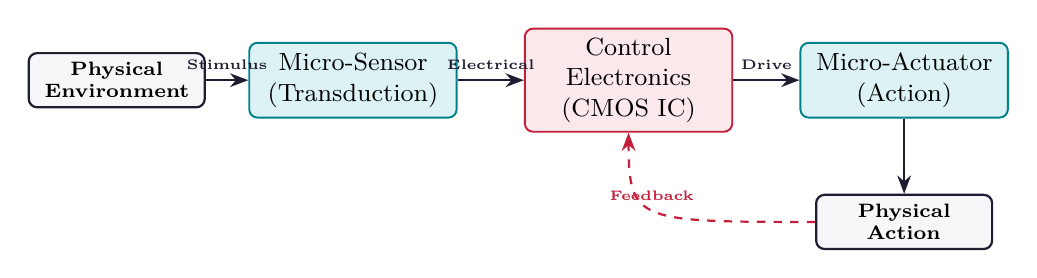
\begin{tikzpicture}[node distance=1.4cm, thick]
  % Nodes
  \node[rectangle, draw=mydark, fill=mygray, rounded corners=3pt, text width=2.0cm, align=center, font=\scriptsize\bfseries] (env) at (-5.0, 0) {Physical\\Environment};
  
  \node[block] (sensor) at (-2.0, 0) {Micro-Sensor\\(Transduction)};
  
  \node[rectangle, draw=myred, fill=hdrred, rounded corners=3pt, text width=2.4cm, align=center, minimum height=0.95cm, font=\small, line width=0.7pt] (control) at (1.5, 0) {Control\\Electronics\\(CMOS IC)};
  
  \node[block] (actuator) at (5.0, 0) {Micro-Actuator\\(Action)};
  
  \node[rectangle, draw=mydark, fill=mygray, rounded corners=3pt, text width=2.0cm, align=center, font=\scriptsize\bfseries] (action) at (5.0, -1.8) {Physical\\Action};

  % Connections
  \draw[arrow] (env) -- (sensor) node[midway, above, font=\tiny\bfseries] {Stimulus};
  \draw[arrow] (sensor) -- (control) node[midway, above, font=\tiny\bfseries] {Electrical};
  \draw[arrow] (control) -- (actuator) node[midway, above, font=\tiny\bfseries] {Drive};
  \draw[arrow] (actuator) -- (action);
  
  % Feedback loop
  \draw[redarrow, dashed] (action.west) .. controls (1.5, -1.8) .. (control.south) node[midway, above, font=\tiny\bfseries] {Feedback};
\end{tikzpicture}
\end{tcolorbox}

% ===============================================================================
\section{History and Milestones of Miniaturization}
% ===============================================================================

The evolution of MEMS spans several decades, transitioning from basic laboratory micro-mechanical discoveries to commercial monolithic consumer electronic devices.

\subsection{Richard Feynman's Vision (1959)}
The conceptual foundation of nanotechnology and micro-manufacturing was laid by physicist Richard Feynman on December 29, 1959, during his famous American Physical Society lecture at Caltech: \textit{"There's Plenty of Room at the Bottom"}.
\textbf{Key Concepts Proposed by Feynman:}
\begin{itemize}[leftmargin=*, itemsep=2.5pt]
  \item \textbf{Writing at Atomic Scale:} Suggested writing the entire 24 volumes of the Encyclopaedia Britannica on the head of a pin by scaling down the font size.
  \item \textbf{Micro-machining Tools:} Envisioned building micro-scale mechanical hands that could build even smaller machines, cascading down to build atomic-scale factories.
  \item \textbf{MEMS Actuators:} Proposed the creation of tiny motors (micro-motors) and electrostatic actuators using micro-lithographic techniques.
  \item \textbf{Physical Scaling:} Highlighted that as machines scale down, the relative importance of physical forces changes (gravity fades, while surface tension and electrostatic forces dominate).
\end{itemize}

\subsection{Key Historical Milestones}
The realization of Feynman's vision was enabled by the development of silicon semiconductor manufacturing and micromachining processes:
\begin{itemize}[leftmargin=*, itemsep=4pt]
  \item \textbf{1954 --- Discovery of Piezoresistivity in Silicon:} C. S. Smith discovered that silicon exhibits a large change in electrical resistance when mechanical stress is applied. This made silicon an exceptional material for pressure and strain sensors.
  \item \textbf{1967 --- Resonant Gate Transistor (RGT):} Developed by Harvey Nathanson at Westinghouse. It was the first batch-fabricated MEMS device, utilizing a moving gold cantilever beam acting as the gate element of a MOS transistor.
  \item \textbf{1970s --- Silicon Bulk Micromachining:} Techniques for anisotropic chemical etching of silicon (using KOH) were perfected, enabling the production of thin silicon membranes for pressure sensors.
  \item \textbf{1980s --- Surface Micromachining:} R. T. Howe and R. S. Muller at UC Berkeley developed surface micromachining. They used polysilicon as the structural material and silicon dioxide ($SiO_2$) as the sacrificial material to release free-moving mechanical structures like micro-cantilevers and gears.
  \item \textbf{1989 --- Electrostatic Comb Drive:} Developed by W. C. Tang, T. H. Nguyen, and R. T. Howe. It introduced lateral comb structures that generate electrostatic forces, forming the basis of micro-resonators and gyroscopes.
  \item \textbf{1990s --- Commercialization and DRIE:} The invention of Deep Reactive Ion Etching (DRIE) by the Bosch Process enabled etching of high-aspect-ratio trenches in silicon. Commercialization succeeded with ADI's ADXL50 accelerometer (for automotive airbag deployment) and TI's Digital Micromirror Device (DMD) for projectors.
\end{itemize}

% ===============================================================================
\section{Applications of MEMS}
% ===============================================================================

MEMS technology is ubiquitous across several key industrial sectors:

\subsection{Automotive Industry}
The automotive sector was the primary driver of MEMS commercialization, requiring high reliability and low-cost sensor components.
\begin{itemize}[leftmargin=*, itemsep=3pt]
  \item \textbf{Airbag Accelerometers:} Capable of measuring sudden deceleration ($50\text{ g}$ to $100\text{ g}$) to deploy airbags within milliseconds.
  \item \textbf{Electronic Stability Control (ESC):} Uses MEMS gyroscopes and accelerometers to measure vehicle yaw rate and lateral acceleration, applying differential braking to prevent skids.
  \item \textbf{Tire Pressure Monitoring Systems (TPMS):} Wireless piezoresistive pressure sensors mounted inside the tires to monitor inflation levels.
\end{itemize}

\subsection{Consumer Electronics}
MEMS enabled the miniaturization and touch interface revolution in personal devices.
\begin{itemize}[leftmargin=*, itemsep=3pt]
  \item \textbf{Smartphones:} Utilize 3-axis MEMS accelerometers (screen auto-rotation), gyroscopes (mobile gaming, stabilization), and MEMS barometers (altitude tracking).
  \item \textbf{MEMS Microphones:} Capacitive micro-scale microphones replacing traditional electret condenser microphones (ECM), offering better sound quality, thermal stability, and noise cancellation.
  \item \textbf{Display Systems (TI DMD):} Digital Micromirror Devices contain millions of microscopic electrostatic mirrors on a single chip, controling light reflections for digital cinema projectors.
\end{itemize}

\subsection{Medical and Biomedical (Bio-MEMS)}
The intersection of MEMS and biomedical engineering has created a new class of diagnostics and therapy.
\begin{itemize}[leftmargin=*, itemsep=3pt]
  \item \textbf{Disposable Pressure Sensors:} Piezoresistive catheter tip sensors used for real-time arterial blood pressure monitoring during surgeries.
  \item \textbf{Lab-on-a-Chip (LoC):} Microfluidic channels, pumps, and valves integrated on a chip to perform complex blood analysis and DNA profiling rapidly with microliters of sample.
  \item \textbf{Microneedles and Drug Delivery:} Array of silicon microneedles ($100\ \mu\text{m}$ to $500\ \mu\text{m}$ long) that penetrate the outer dead skin layer painlessly to deliver transdermal drug therapies.
\end{itemize}

\newpage
% ===============================================================================
% MANDATORY QUICK REVISION PAGE
% ===============================================================================
\begin{center}
  {\large\bfseries\color{myred} Quick Revision --- Module I}\\[3pt]
  {\small\color{mydark} Introduction and Historical Background $|$ PE-EC603A}
\end{center}
\noindent{\color{myred}\rule{\linewidth}{1.2pt}}
\vspace{4pt}

\begin{tcolorbox}[formulabox, title={\textbf{Key Concepts and Parameters}}]
\renewcommand{\arraystretch}{1.3}
\begin{tabularx}{\linewidth}{B{3.8cm} X}
Aspect Ratio (AR)        & $\text{Aspect Ratio} = \displaystyle\frac{\text{Height } (h)}{\text{Width } (w)}$ \\[8pt]
Feynman's Scaling Rule   & $F \propto L^n$ \quad (Forces scale down differently depending on $n$) \\[4pt]
Piezoresistive Effect    & $\displaystyle\frac{\Delta R}{R} = G \cdot \epsilon$ \quad ($G$ = Gauge Factor, $\epsilon$ = Mechanical Strain)
\end{tabularx}
\end{tcolorbox}

\begin{tcolorbox}[defbox, title={\textbf{One-Line Definitions}}]
\begin{itemize}[leftmargin=*, itemsep=2.5pt, topsep=0pt]
  \item \textbf{MEMS:} Micro-scale integrated systems combining mechanical, electrical, and control functions on a single silicon chip.
  \item \textbf{Microsystem:} An engineering system containing sensors, actuators, and electronics to bridge the physical and electrical domains.
  \item \textbf{Aspect Ratio:} The ratio of the height of a microfabricated structure to its lateral width.
  \item \textbf{Piezoresistivity:} The change in electrical resistivity of a material (especially silicon) under applied mechanical stress.
  \item \textbf{Sacrificial Layer:} A temporary film layer ($SiO_2$) deposited during surface micromachining, etched away later to release moving parts.
  \item \textbf{Structural Layer:} The functional, moving material layer (usually Polysilicon) that forms the core device structure in surface micromachining.
  \item \textbf{DRIE:} Deep Reactive Ion Etching, an anisotropic dry etching process used to fabricate high-aspect-ratio silicon trenches.
\end{itemize}
\end{tcolorbox}

\begin{tcolorbox}[exambox, title={\textbf{Frequently Asked / Viva Questions}}]
\begin{enumerate}[topsep=0pt, label=\textbf{Q\arabic*.}, itemsep=5pt]
  \item \Q{What is the primary difference between a sensor and an actuator in a MEMS device?}
    A sensor converts physical variables (e.g., pressure, acceleration) into electrical signals. An actuator converts electrical signals into physical motion or action (e.g., micro-mirror tilt, micro-valve opening).
  \item \Q{How did C. S. Smith's 1954 discovery of piezoresistivity influence MEMS technology?}
    Smith's discovery showed that silicon's resistance changes significantly under stress, forming the transduction basis for pressure sensors, accelerometers, and strain gauges.
  \item \Q{Why did Richard Feynman's 1959 speech serve as the conceptual basis for MEMS?}
    Feynman predicted that machines could be scaled down, that micro-machining could build micro-motors, and that physical scaling would shift dominance from gravity to electrostatic and surface forces.
  \item \Q{What is the structural role of a sacrificial layer in surface micromachining?}
    It acts as a temporary spacer supporting the structural layer during deposition. Once etched away (released) with an acid, it leaves the structural layer suspended and free to move.
  \item \Q{Why is single-crystal silicon the dominant substrate material in MEMS?}
    Silicon has excellent mechanical properties: no mechanical hysteresis, high fatigue strength, can be easily batch-fabricated using established CMOS semiconductor facilities.
  \item \Q{What was the Resonant Gate Transistor (RGT) and why was it a milestone?}
    Developed in 1967, it was the first batch-fabricated MEMS device. It used a moving gold cantilever as a transistor gate, proving mechanical elements could be integrated with microelectronics.
  \item \Q{Why is packaging more complex for MEMS devices compared to standard Integrated Circuits (ICs)?}
    ICs are hermetically sealed from the environment. MEMS sensors must interface directly with external media (like air or fluid) while simultaneously protecting sensitive control electronics.
  \item \Q{Explain the function of a MEMS gyroscope in consumer electronics.}
    It measures the angular rate of rotation (yaw, pitch, roll), enabling camera image stabilization, vehicular electronic stability control, and smartphone motion controls.
  \item \Q{What is LIGA technology and when is it preferred?}
    LIGA is a German acronym for lithography, electroplating, and molding. It uses high-energy X-ray lithography to fabricate structures with extremely high aspect ratios.
  \item \Q{State two applications of Bio-MEMS.}
    Disposable catheter tip blood pressure sensors and Lab-on-a-Chip (LoC) microsystems for rapid blood diagnosis and DNA sequencing.
  \item \Q{How does a MEMS accelerometer in an automotive airbag sensor function?}
    A suspended proof mass deflects under sudden deceleration, changing the capacitance between moving and fixed electrodes to trigger the airbag within milliseconds.
\end{enumerate}
\end{tcolorbox}

\begin{tcolorbox}[tikzbox, title={Comparison: Silicon (MEMS) vs. Steel (Macro-engineering)}]
\renewcommand{\arraystretch}{1.45}
\par\noindent
\begin{tabularx}{\linewidth}{|B{3.2cm}|Y|Y|}
\hline
\textbf{Property} & \textbf{\color{myteal}Silicon (Si)} & \textbf{\color{myamber}Structural Steel} \\
\hline
\textbf{Yield Strength} & $7\text{ GPa}$ (higher than steel). & $0.2 - 0.5\text{ GPa}$. \\
\hline
\textbf{Young's Modulus} & $190\text{ GPa}$ (stiff, similar to steel). & $200\text{ GPa}$. \\
\hline
\textbf{Mechanical Hysteresis} & Negligible (extremely elastic). & Significant (plastic deformation). \\
\hline
\textbf{Fatigue Lifetime} & Infinite (no dislocation movement under stress). & Finite (dislocations accumulate, causing fracture). \\
\hline
\textbf{Density} & $2.3\text{ g/cm}^3$ (lightweight). & $7.8\text{ g/cm}^3$. \\
\hline
\end{tabularx}
\end{tcolorbox}


% -- Module 2 -----------------------------------------------------------------
\modulestart{2}{Geometric Scaling Laws}

\section{Geometric Scaling Laws}
% ===============================================================================

Scaling laws describe how the physical properties of a system change when its physical dimensions are scaled down. In micro-electro-mechanical systems (MEMS), scaling down the linear dimensions changes the relative importance of different physical phenomena.

\subsection{Linear Scale Parameter and Scaling Factor}
Let $L$ denote the characteristic linear scale parameter (dimension) of a device. 
\begin{tcolorbox}[defbox]
\textbf{Scaling Factor ($s$):} The ratio of the scaled-down dimension ($l$) to the original reference dimension ($L$):
$$s = \frac{l}{L}$$
A physical parameter $P$ that scales with the $n$-th power of the linear dimension $L$ is represented as:
$$P \propto L^n \quad \implies \quad \frac{P_{\text{new}}}{P_{\text{old}}} = s^n$$
where $n$ is the scaling exponent.
\end{tcolorbox}

\subsection{Surface Area vs. Volume Scaling}
For a cube of side length $L$:
\begin{itemize}[leftmargin=*, itemsep=3pt]
  \item \textbf{Surface Area ($A$):} $A = 6L^2 \propto L^2$. Scaling factor: $[s^2]$.
  \item \textbf{Volume ($V$):} $V = L^3 \propto L^3$. Scaling factor: $[s^3]$.
\end{itemize}

\subsection{Surface-to-Volume Ratio \texorpdfstring{($S/V$)}{S/V}}
The surface-to-volume ratio of a system of size $L$ is:
$$\frac{S}{V} = \frac{6L^2}{L^3} = \frac{6}{L} \propto L^{-1}$$
Scaling factor: $[s^{-1}]$.

\textbf{Physical Implication:}
As a structure shrinks (e.g., $s = 10^{-3}$, scaling from $1\text{ mm}$ to $1\ \mu\text{m}$):
\begin{itemize}[leftmargin=*, itemsep=2.5pt]
  \item The volume (and mass) decreases by a factor of $10^9$ ($s^3$).
  \item The surface area decreases by a factor of $10^6$ ($s^2$).
  \item The surface-to-volume ratio increases by a factor of $1000$ ($s^{-1}$).
\end{itemize}
Therefore, at the micro-scale, all physical phenomena that depend on surface area (e.g., electrostatic forces, surface tension, viscous drag, heat conduction) dominate over phenomena that depend on volume or mass (e.g., gravity, inertia, magnetic force).

\subsection{Visualizing Cube Scaling}
The following diagram demonstrates the geometric scaling of a block.

\begin{tcolorbox}[tikzbox, title={Comparison of Geometric Scaling}]
\centering
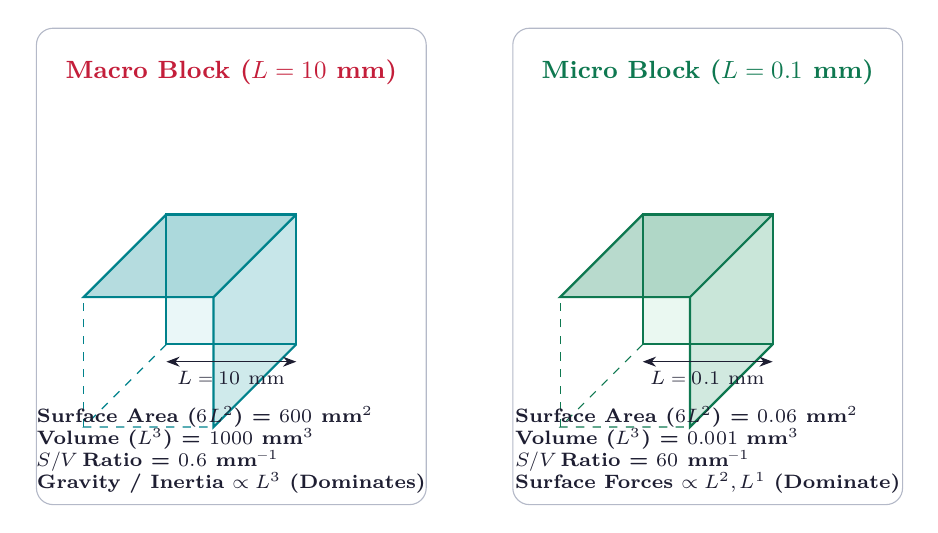
\begin{tikzpicture}[x=0.55cm, y=0.55cm, z=0.35cm, >=Stealth]
  % Card container 1 (Macro-scale)
  \begin{scope}[shift={(-5.5,0)}]
    \draw[fill=white, draw=mgframe, rounded corners=6pt] (-4.5,-5.2) rectangle (4.5,5.8);
    \node[anchor=north, font=\small\bfseries\color{myred}] at (0,5.3) {Macro Block ($L = 10\text{ mm}$)};
    
    % Draw 3D Cube
    \coordinate (O1) at (-1.5,-1.5,0);
    \coordinate (A1) at (1.5,-1.5,0);
    \coordinate (B1) at (1.5,1.5,0);
    \coordinate (C1) at (-1.5,1.5,0);
    \coordinate (D1) at (-1.5,-1.5,-3);
    \coordinate (E1) at (1.5,-1.5,-3);
    \coordinate (F1) at (1.5,1.5,-3);
    \coordinate (G1) at (-1.5,1.5,-3);
    
    \fill[hdrteal, opacity=0.6] (O1) -- (A1) -- (B1) -- (C1) -- cycle;
    \fill[hdrteal!80!myteal, opacity=0.6] (A1) -- (E1) -- (F1) -- (B1) -- cycle;
    \fill[hdrteal!60!myteal, opacity=0.6] (C1) -- (B1) -- (F1) -- (G1) -- cycle;
    
    \draw[myteal, thick] (O1) -- (A1) -- (B1) -- (C1) -- cycle;
    \draw[myteal, thick] (A1) -- (E1) -- (F1) -- (B1);
    \draw[myteal, thick] (C1) -- (G1) -- (F1);
    \draw[myteal, dashed] (O1) -- (D1) -- (E1);
    \draw[myteal, dashed] (D1) -- (G1);
    
    \draw[<->, mydark, thin] ($(O1)-(0,0.4)$) -- ($(A1)-(0,0.4)$) node[midway, below, font=\scriptsize] {$L = 10\text{ mm}$};
    
    \node[anchor=north, align=left, font=\scriptsize\bfseries\color{mydark}] at (0,-2.7) {
      Surface Area ($6L^2$) = $600\text{ mm}^2$ \\
      Volume ($L^3$) = $1000\text{ mm}^3$ \\
      $S/V$ Ratio = $0.6\text{ mm}^{-1}$ \\
      Gravity / Inertia $\propto L^3$ (Dominates)
    };
  \end{scope}

  % Card container 2 (Micro-scale)
  \begin{scope}[shift={(5.5,0)}]
    \draw[fill=white, draw=mgframe, rounded corners=6pt] (-4.5,-5.2) rectangle (4.5,5.8);
    \node[anchor=north, font=\small\bfseries\color{mygreen}] at (0,5.3) {Micro Block ($L = 0.1\text{ mm}$)};
    
    % Draw 3D Cube (visually identical but labeled differently to show scale change)
    \coordinate (O2) at (-1.5,-1.5,0);
    \coordinate (A2) at (1.5,-1.5,0);
    \coordinate (B2) at (1.5,1.5,0);
    \coordinate (C2) at (-1.5,1.5,0);
    \coordinate (D2) at (-1.5,-1.5,-3);
    \coordinate (E2) at (1.5,-1.5,-3);
    \coordinate (F2) at (1.5,1.5,-3);
    \coordinate (G2) at (-1.5,1.5,-3);
    
    \fill[hdrgreen, opacity=0.6] (O2) -- (A2) -- (B2) -- (C2) -- cycle;
    \fill[hdrgreen!80!mygreen, opacity=0.6] (A2) -- (E2) -- (F2) -- (B2) -- cycle;
    \fill[hdrgreen!60!mygreen, opacity=0.6] (C2) -- (B2) -- (F2) -- (G2) -- cycle;
    
    \draw[mygreen, thick] (O2) -- (A2) -- (B2) -- (C2) -- cycle;
    \draw[mygreen, thick] (A2) -- (E2) -- (F2) -- (B2);
    \draw[mygreen, thick] (C2) -- (G2) -- (F2);
    \draw[mygreen, dashed] (O2) -- (D2) -- (E2);
    \draw[mygreen, dashed] (D2) -- (G2);
    
    \draw[<->, mydark, thin] ($(O2)-(0,0.4)$) -- ($(A2)-(0,0.4)$) node[midway, below, font=\scriptsize] {$L = 0.1\text{ mm}$};
    
    \node[anchor=north, align=left, font=\scriptsize\bfseries\color{mydark}] at (0,-2.7) {
      Surface Area ($6L^2$) = $0.06\text{ mm}^2$ \\
      Volume ($L^3$) = $0.001\text{ mm}^3$ \\
      $S/V$ Ratio = $60\text{ mm}^{-1}$ \\
      Surface Forces $\propto L^2, L^1$ (Dominate)
    };
  \end{scope}
\end{tikzpicture}
\end{tcolorbox}

% ===============================================================================
\section{Scaling of Physical Forces}
% ===============================================================================

To design micro-actuators and micro-sensors, we must analyze how different physical forces scale down.

\subsection{Gravity and Inertial Forces}
The mass of an object is $m = \rho V \propto L^3$. The gravitational force is:
$$F_g = m g = \rho V g \propto L^3$$
Scaling factor: $[s^3]$.

\textbf{Inertial Force ($F_i$):} Under constant acceleration $a$, $F_i = m a \propto L^3$. Scaling factor: $[s^3]$.

\textbf{Implication:} As dimensions shrink by $10$ times ($s=0.1$), gravity and inertia drop by $1000$ times. At the micro-scale, gravity becomes negligible. Dust mites can walk on walls because gravitational pull is far weaker than surface adhesion.

\subsection{Electrostatic Force}
For a parallel-plate actuator with plate area $A$, plate separation $d$, and applied voltage $V$:
$$F_e = \frac{1}{2} \frac{\epsilon A V^2}{d^2} \propto \frac{L^2 V^2}{L^2} \propto V^2$$
The scaling behavior depends on how the voltage $V$ is scaled:

\subsubsection{Case A: Constant Voltage Scaling \texorpdfstring{($V \propto L^0$)}{V propto L0}}
If the voltage $V$ remains constant while scaling the physical dimensions ($A \propto L^2$, $d \propto L^1$):
$$F_e \propto \frac{L^2 \cdot (1)^2}{L^2} \propto L^0 = 1$$
Scaling factor: $[s^0]$.

\textbf{Implication:} The electrostatic force remains completely constant as the device scales down. This makes electrostatic actuators highly efficient at small scales.

\subsubsection{Case B: Constant Electric Field Scaling \texorpdfstring{($E = V/d = \text{const} \implies V \propto L^1$)}{E = V/d = const => V propto L1}}
To prevent dielectric breakdown in air, the electric field $E$ must be kept constant, meaning the voltage $V$ is scaled down proportionally with gap distance $d$ ($V \propto L^1$):
$$F_e \propto \frac{L^2 \cdot (L)^2}{L^2} \propto L^2$$
Scaling factor: $[s^2]$.

\textbf{Comparison with Gravity:}
$$\frac{F_e}{F_g} \propto \frac{L^2}{L^3} \propto L^{-1}$$
As $L \to \mu\text{m}$ range, the ratio $\frac{F_e}{F_g}$ becomes extremely large, proving that electrostatic forces are orders of magnitude stronger than gravity at micro-scale.

\subsection{Electromagnetic Force}
For an electromagnetic actuator, the magnetic force on a current-carrying conductor of length $l$ in a magnetic field $B$ is:
$$F_m = I (l \times B) \propto I \cdot L \cdot B$$
Let us assume constant current density $J = I / A_{\text{wire}} = \text{const}$, which implies the current scales as $I \propto A_{\text{wire}} \propto L^2$.
The magnetic field $B$ generated by a micro-coil scales as $B \propto \frac{N I}{L} \propto \frac{1 \cdot L^2}{L} \propto L^1$.
$$F_m \propto (L^2) \cdot (L^1) \cdot (L^1) \propto L^4$$
Scaling factor: $[s^4]$.

If permanent magnets are used where $B \propto L^0$ (constant magnetic flux density):
$$F_m \propto I \cdot L \cdot B \propto (L^2) \cdot (L^1) \cdot (1) \propto L^3$$
Scaling factor: $[s^3]$.

\textbf{Implication:} Magnetic coil forces scale as $L^4$, meaning they disappear extremely fast as scale decreases. Hence, magnetic actuators are rarely used in MEMS, unless permanent magnets are integrated.

\subsection{Surface Tension Force}
Surface tension force acts along the contact perimeter $P$ of a fluid interface:
$$F_s = \gamma P \sin\theta \propto L^1$$
where $\gamma$ is the surface tension coefficient ($N/m$), and $P$ is perimeter ($\propto L^1$).
Scaling factor: $[s^1]$.

\textbf{Comparison with Gravity:}
$$\frac{F_s}{F_g} \propto \frac{L^1}{L^3} \propto L^{-2}$$
At $L = 10\ \mu\text{m}$, surface tension forces are $10^8$ times stronger than gravity. This leads to stiction, where moving micro-structures stick to the substrate during liquid-based etching releases.

% ===============================================================================
\section{Fluidic and Thermal Scaling}
% ===============================================================================

Scaling down also changes heat and fluid transport physics.

\subsection{Fluidic Scaling: Reynolds Number \texorpdfstring{($Re$)}{Re}}
The Reynolds number determines the flow regime (laminar vs. turbulent) of a fluid in a channel:
\begin{tcolorbox}[formulabox, title={Reynolds Number Scaling}]
$$Re = \frac{\rho v D_h}{\mu}$$
where:
\begin{tabular}{lcl}
$\rho$ & = & density of fluid ($kg/m^3$) $\propto L^0$ \\
$v$ & = & flow velocity ($m/s$) $\propto L^0$ (assumed constant) \\
$D_h$ & = & hydraulic diameter of the channel ($m$) $\propto L^1$ \\
$\mu$ & = & dynamic viscosity of fluid ($Pa \cdot s$) $\propto L^0$
\end{tabular}
\end{tcolorbox}
Therefore:
$$Re \propto L^1$$
Scaling factor: $[s^1]$.

\textbf{Physical Consequences in Microfluidics:}
\begin{itemize}[leftmargin=*, itemsep=2.5pt]
  \item In macro-scale pipes, $Re > 4000$ (turbulent flow, dominant inertia).
  \item In micro-channels ($D_h \approx 50\ \mu\text{m}$), $Re \ll 1$ (typically $0.1$ to $10$).
  \item \textbf{Strict Laminar Flow:} At low $Re$, fluid flows in parallel streams without mixing. Turbulent mixing is impossible.
  \item \textbf{Diffusion Mixing:} Mixing occurs only via passive molecular diffusion. The diffusion time $t$ scales as:
  $$t \propto \frac{x^2}{D} \propto L^2$$
  Since the diffusion distance $x \approx L$ is extremely small in micro-channels, mixing by diffusion is fast enough for practical microfluidic applications, despite the laminar regime.
\end{itemize}

\subsection{Thermal Scaling}
Let us analyze heat transfer by conduction through a medium of area $A$, thickness $d \approx L$, and thermal conductivity $k$:
\begin{itemize}[leftmargin=*, itemsep=3.5pt]
  \item \textbf{Heat Conduction Flow Rate ($q$):}
  $$q = -k A \frac{\Delta T}{d} \propto \frac{L^2}{L^1} \propto L^1$$
  Scaling factor: $[s^1]$.
  \item \textbf{Thermal Resistance ($R_{\text{th}}$):}
  $$R_{\text{th}} = \frac{d}{k A} \propto \frac{L}{L^2} \propto L^{-1}$$
  Scaling factor: $[s^{-1}]$.
  \item \textbf{Heat Capacity ($C_{\text{th}}$):}
  $$C_{\text{th}} = m c_p = \rho V c_p \propto L^3$$
  Scaling factor: $[s^3]$.
  \item \textbf{Thermal Time Constant ($\tau_{\text{th}}$):}
  $$\tau_{\text{th}} = R_{\text{th}} C_{\text{th}} \propto L^{-1} \cdot L^3 \propto L^2$$
  Scaling factor: $[s^2]$.
\end{itemize}

\textbf{Implication:}
The thermal time constant scales as $L^2$. If a thermal actuator is scaled down by a factor of 100 ($s = 0.01$):
$$\frac{\tau_{\text{new}}}{\tau_{\text{old}}} = s^2 = 10^{-4}$$
The device heats and cools $10,000$ times faster. MEMS thermal sensors and actuators can operate in the microsecond range, making them highly responsive.

\newpage
% ===============================================================================
% MANDATORY QUICK REVISION PAGE
% ===============================================================================
\begin{center}
  {\large\bfseries\color{myred} Quick Revision --- Module II}\\[3pt]
  {\small\color{mydark} Scaling Effects in Microsystems $|$ PE-EC603A}
\end{center}
\noindent{\color{myred}\rule{\linewidth}{1.2pt}}
\vspace{4pt}

\begin{tcolorbox}[formulabox, title={\textbf{Summary of Scaling Laws}}]
\renewcommand{\arraystretch}{1.3}
\begin{tabularx}{\linewidth}{B{3.8cm} Y Y}
\textbf{Physical Parameter} & \textbf{Formula / Definition} & \textbf{Scaling Exponent ($n$ in $L^n$)} \\
\hline
Surface-to-Volume Ratio & $S/V = 6/L$ & $n = -1$ \\
Gravity / Mass Force & $F_g = \rho V g$ & $n = 3$ \\
Electrostatic Force (Const $V$) & $F_e = \frac{1}{2} \epsilon A V^2 / d^2$ & $n = 0$ \\
Electrostatic Force (Const $E$) & $F_e \propto L^2 E^2$ & $n = 2$ \\
Electromagnetic Force (Coil) & $F_m \propto I L B$ & $n = 4$ \\
Surface Tension Force & $F_s = \gamma P$ & $n = 1$ \\
Reynolds Number & $Re = \rho v D_h / \mu$ & $n = 1$ \\
Thermal Time Constant & $\tau_{\text{th}} = R_{\text{th}} C_{\text{th}}$ & $n = 2$ \\
\end{tabularx}
\end{tcolorbox}

\begin{tcolorbox}[defbox, title={\textbf{One-Line Definitions}}]
\begin{itemize}[leftmargin=*, itemsep=2.5pt, topsep=0pt]
  \item \textbf{Scaling Law:} An equation that predicts how a physical quantity changes when the characteristic size of the system is altered.
  \item \textbf{Surface-to-Volume Ratio ($S/V$):} The ratio of external boundary area to internal volume; it scales as $L^{-1}$ and dominates micro-scale transport.
  \item \textbf{Constant Voltage Scaling:} A micro-scaling method where system voltages are kept constant, resulting in constant electrostatic force ($L^0$).
  \item \textbf{Constant Field Scaling:} A scaling approach where electric field is kept constant to prevent dielectric breakdown, scaling voltage as $L^1$ and force as $L^2$.
  \item \textbf{Reynolds Number ($Re$):} A dimensionless ratio of inertial forces to viscous forces; it scales as $L^1$ and is very small in microsystems.
  \item \textbf{Laminar Flow:} A flow regime characterized by smooth, parallel fluid layers with zero turbulence; occurs when $Re \ll 2000$.
  \item \textbf{Thermal Time Constant ($\tau_{\text{th}}$):} The measure of thermal response speed; scales as $L^2$, enabling microsecond thermal operations in MEMS.
\end{itemize}
\end{tcolorbox}

\begin{tcolorbox}[exambox, title={\textbf{Frequently Asked / Viva Questions}}]
\begin{enumerate}[topsep=0pt, label=\textbf{Q\arabic*.}, itemsep=5pt]
  \item \Q{Why does the surface-to-volume ratio ($S/V$) increase as a device is scaled down?}
    Because surface area scales as $L^2$ while volume scales as $L^3$. Dividing area by volume yields $S/V \propto L^{-1}$, which approaches infinity as $L$ approaches zero.
  \item \Q{Which force dominates: electrostatic or electromagnetic at the micro-scale, and why?}
    Electrostatic force dominates. Under constant voltage scaling, electrostatic force remains constant ($L^0$), whereas magnetic coil forces scale as $L^4$. Thus, electrostatic actuators are vastly superior at the microscale.
  \item \Q{Why is constant voltage scaling preferred over constant field scaling for MEMS actuators?}
    Under constant voltage scaling, the force remains constant ($L^0$). Under constant field scaling, the force drops as $L^2$, reducing performance at smaller sizes.
  \item \Q{What is stiction in surface micromachining and which scaling law causes it?}
    Stiction is the permanent sticking of released micro-beams to the substrate. It is caused by capillary surface tension forces, which scale as $L^1$, dominating gravity ($L^3$) during the wet-release drying process.
  \item \Q{Why is it impossible to create turbulent mixing inside a standard microfluidic channel?}
    Because the hydraulic diameter ($D_h \propto L^1$) is tiny, resulting in a very low Reynolds number ($Re \propto L^1 \ll 1$). At such low values, flow is strictly laminar and turbulence cannot form.
  \item \Q{How do fluids mix in a microfluidic channel if the flow is strictly laminar?}
    Mixing occurs entirely via molecular diffusion. Because diffusion distances are extremely small, diffusion times (which scale as $t \propto L^2$) are short enough to allow rapid mixing.
  \item \Q{Why do MEMS thermal actuators have extremely fast response times?}
    The thermal time constant $\tau_{\text{th}}$ scales as $L^2$. Decreasing dimensions by a factor of 100 reduces the heating/cooling response time by a factor of 10,000.
  \item \Q{How does magnetic force scale for permanent magnets in MEMS?}
    Since the magnetic flux density $B$ of a permanent magnet scales as $L^0$, the force scales as $F_m \propto I L B \propto (L^2)(L^1)(1) \propto L^3$. This is better than coil-based magnetic forces ($L^4$).
  \item \Q{Why do dust particles float in air while stones fall quickly?}
    For a stone (macro-scale), weight ($L^3$) dominates over air resistance ($L^2$). For dust (micro-scale), weight is negligible, and surface drag dominates, keeping the particle suspended.
  \item \Q{Explain the scaling of heat conduction flow rate.}
    According to Fourier's law, heat conduction rate $q = -k A \frac{\Delta T}{d}$. Since area $A \propto L^2$ and distance $d \propto L^1$, the heat flow rate $q$ scales as $L^1$.
  \end{enumerate}
\end{tcolorbox}

\begin{tcolorbox}[tikzbox, title={Actuator Scaling Law Comparison Summary}]
\renewcommand{\arraystretch}{1.45}
\par\noindent
\begin{tabularx}{\linewidth}{|B{3.2cm}|Y|Y|Y|}
\hline
\textbf{Actuation Mode} & \textbf{Scaling Exponent ($n$)} & \textbf{Strength at Macro-scale} & \textbf{Strength at Micro-scale} \\
\hline
\textbf{Electrostatic (Const $V$)} & $n = 0$ (Constant) & Weak (requires high voltages for macro effects). & Very Strong (dominates device behavior). \\
\hline
\textbf{Electrostatic (Const $E$)} & $n = 2$ & Moderate. & Strong. \\
\hline
\textbf{Electromagnetic (Coil)} & $n = 4$ & Very Strong (motors, solenoids). & Extremely Weak (impractical for MEMS). \\
\hline
\textbf{Piezoelectric} & $n = 2$ & Strong. & High force but small stroke. \\
\hline
\textbf{Thermal Bimorph} & $n = 1$ (Speed $\propto L^2$) & Slow. & Extremely Fast, high force. \\
\hline
\end{tabularx}
\tcbset{breakable}
\end{tcolorbox}


% -- Module 3 -----------------------------------------------------------------
\modulestart{3}{MEMS Sensors}

\section{MEMS Sensors}
% ===============================================================================

Sensors are transduction elements that convert mechanical, thermal, optical, chemical, or biological signals from the physical environment into electrical outputs.

\subsection{Piezoresistive Sensors}
Piezoresistivity is the change in electrical resistivity ($\rho$) of a material when subjected to mechanical strain.
\begin{tcolorbox}[defbox]
\textbf{Gauge Factor ($G$):} The ratio of fractional change in resistance to the mechanical strain ($\epsilon$):
$$G = \frac{\Delta R / R}{\epsilon} = (1 + 2\nu) + \frac{\Delta\rho/\rho}{\epsilon}$$
where $\nu$ is the Poisson's ratio, and $\epsilon$ is the longitudinal strain.
\end{tcolorbox}
In metals, piezoresistivity is primarily due to geometric changes ($1+2\nu \approx 1.6$). In semiconductors like Silicon, it is dominated by band-structure changes under stress ($\Delta\rho/\rho \gg 1+2\nu$), yielding much higher gauge factors ($G \approx 100$ to $200$).

\textbf{Advantages:} High sensitivity, linear response, simple circuitry (Wheatstone bridge interface). \\
\textbf{Disadvantages:} Highly temperature-sensitive (requires compensation), drift over time.

\subsection{Capacitive Sensors}
Capacitive sensors measure changes in capacitance between a moving electrode and a fixed electrode:
$$C = \frac{\epsilon_r \epsilon_0 A}{d}$$

There are two primary modes of capacitive sensing:
\begin{itemize}[leftmargin=*, itemsep=4pt]
  \item \textbf{Gap-closing mode ($d$ changes):}
  $$C(x) = \frac{\epsilon_r \epsilon_0 A}{d_0 - x} \implies \frac{dC}{dx} = \frac{\epsilon_r \epsilon_0 A}{(d_0 - x)^2} \quad \text{(Non-linear, highly sensitive)}$$
  \item \textbf{Overlap-area mode ($A$ changes):}
  $$C(x) = \frac{\epsilon_r \epsilon_0 w (L - x)}{d} \implies \frac{dC}{dx} = -\frac{\epsilon_r \epsilon_0 w}{d} \quad \text{(Strictly linear)}$$
\end{itemize}

\textbf{Advantages:} Low power consumption, high temperature stability, negligible mechanical loading, low noise. \\
\textbf{Disadvantages:} Susceptible to electromagnetic interference (EMI) and parasitic capacitance (requires on-chip electronics).

\subsection{Piezoelectric Sensors}
Piezoelectric materials generate a transient surface charge $Q$ in response to applied force $F$:
$$Q = d_{ij} \cdot F$$
where $d_{ij}$ is the piezoelectric charge coefficient ($C/N$). Common materials include Quartz, Zinc Oxide ($ZnO$), Lead Zirconate Titanate ($PZT$), and Aluminum Nitride ($AlN$).

\textbf{Key Characteristic:} Active/self-generating sensor. It can only measure dynamic changes because static charges leak away through the measurement circuitry.

% ===============================================================================
\section{MEMS Actuators}
% ===============================================================================

Actuators convert electrical energy into mechanical movement or force.

\subsection{Electrostatic Comb Drive Actuators}
Comb drives consist of two interdigitated finger electrodes: one anchored (fixed) and one suspended on a spring (movable).

\begin{tcolorbox}[formulabox, title={Comb Drive Lateral Actuation Force}]
When a voltage $V$ is applied, the lateral force $F_x$ pulling the fingers together is:
$$F_x = N \frac{\epsilon_0 \epsilon_r h}{d} V^2$$
where:
\begin{tabular}{lcl}
$N$ & = & number of finger pairs \\
$h$ & = & thickness (height) of the fingers \\
$d$ & = & gap distance between the interdigitated fingers \\
$V$ & = & applied voltage
\end{tabular}
\end{tcolorbox}

\textbf{Crucial Feature:} The force $F_x$ is independent of lateral displacement $x$. This provides a stable, predictable force over a large range of motion, unlike parallel-plate electrostatic actuators (which suffer from pull-in instability).

\subsection{Thermal Actuators}
Thermal actuators utilize electrical resistive heating (Joule heating, $P = I^2 R$) to produce thermal expansion and generate mechanical movement.

\subsubsection{Thermal Bimorph}
Consists of two bonded layers with different Coefficients of Thermal Expansion ($\text{CTE}_1 > \text{CTE}_2$). Upon heating, the bimorph bends toward the material with the lower CTE (Layer 2).

\subsubsection{Chevron / V-Beam Actuator}
Symmetrical angled silicon beams anchored at the ends. Passing current through the beams causes thermal expansion, which forces the center shuttle forward in a linear direction, magnifying the displacement.

\subsection{Piezoelectric Actuators}
Piezoelectric actuators use the converse piezoelectric effect: applying an electric field $E$ induces mechanical strain $\epsilon = d_{ij} \cdot E$.
\begin{itemize}[leftmargin=*]
  \item \textbf{Stack Actuators:} Multiple thin piezoelectric layers stacked together.
  \item \textbf{Performance:} Extremely high force output, sub-nanometer resolution, but very small displacement (typically $< 0.1\%$ of length).
\end{itemize}

% ===============================================================================
\section{Microfabrication Processes}
% ===============================================================================

MEMS fabrication relies on modifying planar IC manufacturing steps for three-dimensional mechanical structures.

\subsection{Thermal Oxidation \& The Deal-Grove Model}
Thermal oxidation grows Silicon Dioxide ($SiO_2$) on Silicon at high temperatures ($900^{\circ}\text{C}$--$1200^{\circ}\text{C}$).
\begin{itemize}[leftmargin=*, itemsep=3.5pt]
  \item \textbf{Dry Oxidation ($Si + O_2 \to SiO_2$):} Slow growth rate, dense oxide, high dielectric strength. Used for electrical isolation.
  \item \textbf{Wet Oxidation ($Si + 2H_2O \to SiO_2 + 2H_2$):} Fast growth rate, less dense. Used as thick sacrificial layers.
\end{itemize}

\begin{tcolorbox}[defbox, title={The Deal-Grove Model}]
The Deal-Grove model describes the kinetics of thermal oxidation:
$$x_0^2 + A x_0 = B(t + \tau)$$
where $x_0$ is the oxide thickness, $t$ is oxidation time, $B$ is the parabolic rate constant, $B/A$ is the linear rate constant, and $\tau$ is a time shift parameter representing any pre-existing oxide layer.
\end{tcolorbox}

We identify two limiting regimes of the Deal-Grove model:
\begin{enumerate}[leftmargin=*, label=\arabic*., itemsep=3.5pt]
  \item \textbf{Reaction-limited (Linear) Regime (for short times, $t \ll \frac{A^2}{4B}$):}
  Here, $A x_0 \approx B(t + \tau) \implies x_0 \approx \frac{B}{A}(t + \tau)$.
  Oxide growth is limited by the rate of chemical reaction at the $Si$--$SiO_2$ interface.
  \item \textbf{Diffusion-limited (Parabolic) Regime (for long times, $t \gg \frac{A^2}{4B}$):}
  Here, $x_0^2 \approx B t \implies x_0 \approx \sqrt{B t}$.
  Oxide growth is limited by the rate of oxygen diffusing through the already grown oxide layer to reach the Silicon substrate.
\end{enumerate}

\subsection{Deposition Techniques}
\begin{itemize}[leftmargin=*, itemsep=4pt]
  \item \textbf{PVD (Physical Vapor Deposition):}
    \begin{itemize}[leftmargin=*, itemsep=2pt]
      \item \textbf{Thermal Evaporation:} Heating a target material in high vacuum until it evaporates and condenses on the substrate.
      \item \textbf{Sputtering:} Bombarding a target material with heavy inert gas ions ($Ar^+$) in a plasma, ejecting target atoms toward the substrate.
    \end{itemize}
  \item \textbf{CVD (Chemical Vapor Deposition):} Gases react chemically at the substrate surface to deposit a thin film.
    \begin{itemize}[leftmargin=*, itemsep=2pt]
      \item \textbf{LPCVD (Low Pressure CVD):} High temperature ($> 600^{\circ}\text{C}$), high film purity and uniformity. Used to deposit Polysilicon and Silicon Nitride ($Si_3N_4$).
      \item \textbf{PECVD (Plasma Enhanced CVD):} Plasma assists the reaction, allowing low temperature deposition ($200^{\circ}\text{C}$--$400^{\circ}\text{C}$). Used to deposit dielectrics over metal layers.
    \end{itemize}
\end{itemize}

\subsection{Photolithography Process Flow}
Photolithography transfers geometric patterns from a photo-mask to a light-sensitive polymer (photoresist) on the substrate:
\begin{enumerate}[leftmargin=*, label=\arabic*., itemsep=2.5pt]
  \item \textbf{Substrate Preparation:} Clean wafer and apply adhesion promoter (HMDS).
  \item \textbf{Spin Coating:} Spin liquid photoresist at high speed to obtain a uniform thin film.
  \item \textbf{Soft Bake:} Heat wafer ($90^{\circ}\text{C}$--$100^{\circ}\text{C}$) to evaporate solvents and stabilize resist.
  \item \textbf{Alignment and Exposure:} Align mask to wafer and expose to ultraviolet (UV) light.
  \item \textbf{Development:} Immerse wafer in chemical developer to dissolve selective resist regions.
  \item \textbf{Hard Bake:} Heat wafer ($110^{\circ}\text{C}$--$130^{\circ}\text{C}$) to polymerize and harden the remaining resist.
\end{enumerate}

\textbf{Positive vs. Negative Photoresist:}\par\noindent
\begin{tabularx}{\linewidth}{|B{3.2cm}|Y|Y|}
\hline
\textbf{Property} & \textbf{\color{myteal}Positive Photoresist} & \textbf{\color{mygreen}Negative Photoresist} \\
\hline
\textbf{UV Exposure Effect} & Exposed area becomes soluble in developer. & Exposed area polymerizes/cross-links, becoming insoluble. \\
\hline
\textbf{Mask Pattern Copy} & Identical to mask pattern. & Reversal of mask pattern. \\
\hline
\textbf{Resolution} & Extremely high (sub-micron). & Lower (swelling occurs during development). \\
\hline
\textbf{Common Material} & DNQ-Novolac. & SU-8, polyisoprene-based. \\
\hline
\end{tabularx}

\subsection{Etching and LIGA}
\begin{itemize}[leftmargin=*, itemsep=3.5pt]
  \item \textbf{Wet vs. Dry:} Wet etching uses liquid chemicals (high selectivity, isotropic). Dry etching uses gas plasmas (high anisotropy).
  \item \textbf{Isotropic vs. Anisotropic:} Isotropic etches equally in all directions (creates undercuts). Anisotropic etches in a preferred direction (vertical walls).
  \item \textbf{LIGA:} A German acronym for Lithographie, Galvanoformung, Abformung (Lithography, Electroplating, Molding). Uses synchrotron X-ray source to fabricate metal/plastic components with extremely high aspect ratios ($>100:1$).
\end{itemize}

% ===============================================================================
\section{Surface Micromachining and Stiction}
% ===============================================================================

Surface micromachining builds micro-structures on top of the substrate by depositing and patterning alternating structural and sacrificial layers.

\subsection{Release Etch Sequence}
The most common surface micromachining process uses Silicon as the substrate, Silicon Dioxide ($SiO_2$) as the sacrificial layer, and Polysilicon as the structural material. The sacrificial oxide is removed using hydrofluoric acid (HF) to release the moving polysilicon structures.

\begin{tcolorbox}[tikzbox, title={Surface Micromachining Cantilever Release Sequence}]
\centering
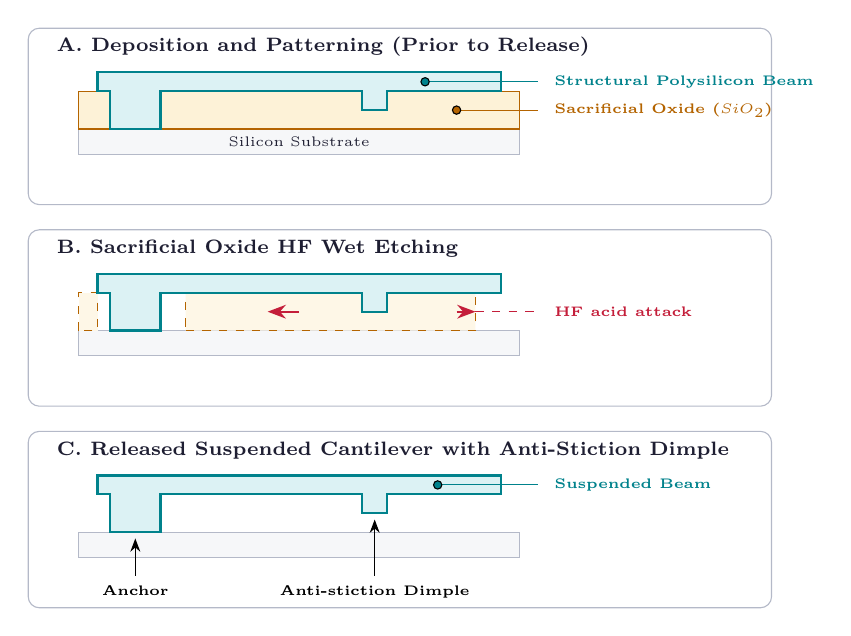
\begin{tikzpicture}[x=0.8cm, y=0.8cm, >=Stealth]
  % STATE 1: Prior to Release
  \begin{scope}[shift={(0,6.4)}]
    \draw[fill=white, draw=mgframe, rounded corners=4pt] (-0.3,-1.2) rectangle (11.5,1.6);
    \node[anchor=west, font=\scriptsize\bfseries\color{mydark}] at (0,1.3) {A. Deposition and Patterning (Prior to Release)};
    % Substrate
    \draw[fill=mygray, draw=mgframe] (0.5,-0.4) rectangle (7.5,0);
    \node[font=\tiny, color=mydark] at (4,-0.2) {Silicon Substrate};
    % Sacrificial Oxide
    \draw[fill=hdramber, draw=myamber] (0.5,0) rectangle (1.0,0.6);
    \draw[fill=hdramber, draw=myamber] (1.8,0) -- (7.5,0) -- (7.5,0.6) -- (5.4,0.6) -- (5.4,0.3) -- (5.0,0.3) -- (5.0,0.6) -- (1.8,0.6) -- cycle;
    % Structural Poly-Si
    \draw[fill=hdrteal, draw=myteal, thick] (0.8,0.6) -- (1.0,0.6) -- (1.0,0) -- (1.8,0) -- (1.8,0.6) -- (5.0,0.6) -- (5.0,0.3) -- (5.4,0.3) -- (5.4,0.6) -- (7.2,0.6) -- (7.2,0.9) -- (0.8,0.9) -- cycle;
    
    % Horizontal Leader Lines and Labels on the right side
    \draw[myteal, thin] (6.0,0.75) -- (7.8,0.75);
    \draw[fill=myteal] (6.0,0.75) circle (1.5pt);
    \node[anchor=west, font=\tiny\bfseries, color=myteal] at (7.9,0.75) {Structural Polysilicon Beam};
    
    \draw[myamber, thin] (6.5,0.3) -- (7.8,0.3);
    \draw[fill=myamber] (6.5,0.3) circle (1.5pt);
    \node[anchor=west, font=\tiny\bfseries, color=myamber] at (7.9,0.3) {Sacrificial Oxide ($SiO_2$)};
  \end{scope}

  % STATE 2: Wet HF Etch Attack
  \begin{scope}[shift={(0,3.2)}]
    \draw[fill=white, draw=mgframe, rounded corners=4pt] (-0.3,-1.2) rectangle (11.5,1.6);
    \node[anchor=west, font=\scriptsize\bfseries\color{mydark}] at (0,1.3) {B. Sacrificial Oxide HF Wet Etching};
    % Substrate
    \draw[fill=mygray, draw=mgframe] (0.5,-0.4) rectangle (7.5,0);
    % Shrinking Oxide (represented with dashed boundaries)
    \draw[fill=hdramber!60, draw=myamber, dashed] (0.5,0) rectangle (0.8,0.6);
    \draw[fill=hdramber!60, draw=myamber, dashed] (2.2,0) -- (6.8,0) -- (6.8,0.6) -- (5.4,0.6) -- (5.4,0.3) -- (5.0,0.3) -- (5.0,0.6) -- (2.2,0.6) -- cycle;
    % Structural Poly-Si
    \draw[fill=hdrteal, draw=myteal, thick] (0.8,0.6) -- (1.0,0.6) -- (1.0,0) -- (1.8,0) -- (1.8,0.6) -- (5.0,0.6) -- (5.0,0.3) -- (5.4,0.3) -- (5.4,0.6) -- (7.2,0.6) -- (7.2,0.9) -- (0.8,0.9) -- cycle;
    % HF Etch arrows
    \draw[redarrow] (4,0.3) -- (3.5,0.3);
    \draw[redarrow] (6.5,0.3) -- (6.8,0.3);
    
    % Leader Line and Label for acid attack
    \draw[myred, thin, dashed] (6.8,0.3) -- (7.8,0.3);
    \node[anchor=west, font=\tiny\bfseries, color=myred] at (7.9,0.3) {HF acid attack};
  \end{scope}

  % STATE 3: Released Structure with Dimple
  \begin{scope}[shift={(0,0)}]
    \draw[fill=white, draw=mgframe, rounded corners=4pt] (-0.3,-1.2) rectangle (11.5,1.6);
    \node[anchor=west, font=\scriptsize\bfseries\color{mydark}] at (0,1.3) {C. Released Suspended Cantilever with Anti-Stiction Dimple};
    % Substrate
    \draw[fill=mygray, draw=mgframe] (0.5,-0.4) rectangle (7.5,0);
    % Structural Poly-Si (Oxide is completely gone)
    \draw[fill=hdrteal, draw=myteal, thick] (0.8,0.6) -- (1.0,0.6) -- (1.0,0) -- (1.8,0) -- (1.8,0.6) -- (5.0,0.6) -- (5.0,0.3) -- (5.4,0.3) -- (5.4,0.6) -- (7.2,0.6) -- (7.2,0.9) -- (0.8,0.9) -- cycle;
    
    % Leader Line and Label for suspended beam
    \draw[myteal, thin] (6.2,0.75) -- (7.8,0.75);
    \draw[fill=myteal] (6.2,0.75) circle (1.5pt);
    \node[anchor=west, font=\tiny\bfseries, color=myteal] at (7.9,0.75) {Suspended Beam};
    
    % Labels below the substrate (within card bounds)
    \draw[<-] (1.4,-0.1) -- (1.4,-0.7) node[below, font=\tiny\bfseries] {Anchor};
    \draw[<-] (5.2,0.2) -- (5.2,-0.7) node[below, font=\tiny\bfseries] {Anti-stiction Dimple};
  \end{scope}
\end{tikzpicture}
\end{tcolorbox}

\subsection{Release Stiction Mechanism}
During drying after wet HF etching, liquid water forms a meniscus between the suspended beam and the substrate.
\begin{enumerate}[leftmargin=*, label=\arabic*.]
  \item As the liquid evaporates, capillary forces (surface tension $F_s \propto L^1$) pull the compliant beam down.
  \item If the beam touches the substrate, solid-solid adhesion forces (van der Waals, hydrogen bonding, electrostatic charge) keep it permanently attached to the substrate. This is called \textbf{Stiction}.
\end{enumerate}

\subsection{Stiction Mitigation Techniques}
\begin{itemize}[leftmargin=*, itemsep=4pt]
  \item \textbf{Anti-stiction Dimples:} Small molded bumps on the underside of the beam (fabricated by etching small shallow pits in the sacrificial oxide prior to structural polysilicon deposition). Dimples reduce the physical contact area by $>98\%$ if the beam collapses, preventing stiction forces from bonding the surfaces.
  \item \textbf{Supercritical CO2 Drying (SCD):} The wet rinsing liquid is replaced with liquid carbon dioxide ($CO_2$). The temperature and pressure are raised above the supercritical point of $CO_2$ ($31.1^{\circ}\text{C}$, $73.9\text{ atm}$), transitioning it directly into gas without a liquid-vapor phase boundary. This completely eliminates surface tension forces, preventing cantilever collapse.
  \item \textbf{Dry Release Processes:} Replacing sacrificial oxide with a polymer layer that is released using an oxygen plasma dry ash, avoiding liquid contact entirely.
\end{itemize}

\newpage
% ===============================================================================
% MANDATORY QUICK REVISION PAGE
% ===============================================================================
\begin{center}
  {\large\bfseries\color{myred} Quick Revision --- Module III}\\[3pt]
  {\small\color{mydark} Sensors, Actuators \& Fabrication $|$ PE-EC603A}
\end{center}
\noindent{\color{myred}\rule{\linewidth}{1.2pt}}
\vspace{4pt}

\begin{tcolorbox}[formulabox, title={\textbf{Key Transduction Formulas}}]
\renewcommand{\arraystretch}{1.3}
\begin{tabularx}{\linewidth}{B{3.8cm} Y Y}
\textbf{Transduction Mechanism} & \textbf{Core Equation} & \textbf{Key Variable Definition} \\
\hline
Piezoresistive Sensitivity & $\displaystyle\frac{\Delta R}{R} = G \cdot \epsilon$ & $G$: Gauge Factor; $\epsilon$: Long strain \\[8pt]
Capacitive Sensitivity (Gap) & $\displaystyle\frac{dC}{dx} = \frac{\epsilon A}{(d_0 - x)^2}$ & $A$: Plate area; $d_0$: Initial gap \\[8pt]
Comb Drive Force (Lateral) & $\displaystyle F_x = N \frac{\epsilon_0 \epsilon_r h}{d} V^2$ & $N$: Finger pairs; $h$: thickness; $d$: gap \\[8pt]
Deal-Grove Kinetics & $x_0^2 + A x_0 = B(t + \tau)$ & $B$: Parabolic rate; $B/A$: Linear rate \\[2pt]
\end{tabularx}
\end{tcolorbox}

\begin{tcolorbox}[defbox, title={\textbf{One-Line Definitions}}]
\begin{itemize}[leftmargin=*, itemsep=2.5pt, topsep=0pt]
  \item \textbf{Gauge Factor ($G$):} The normalized sensitivity of a resistor to mechanical strain; $G_{\text{Silicon}} \gg G_{\text{Metal}}$.
  \item \textbf{Piezoelectric Effect:} The generation of electric charge in response to mechanical stress; utilized in high-frequency resonators.
  \item \textbf{Comb Drive:} An electrostatic actuator utilizing interdigitated fingers to produce constant lateral force.
  \item \textbf{Deal-Grove Model:} A kinetic theory modeling the thermal oxidation rate of silicon under linear and parabolic regimes.
  \item \textbf{Positive Photoresist:} A photo-sensitive polymer that becomes soluble in developer upon UV exposure (e.g., DNQ-Novolac).
  \item \textbf{LIGA:} A micromachining process combining X-ray lithography, electroplating, and molding for extreme aspect ratios.
  \item \textbf{Stiction:} The unwanted permanent adhesion of released micro-mechanical structures to the adjacent substrate.
  \item \textbf{Supercritical Drying:} A drying method eliminating capillary collapse by evaporating $CO_2$ above its supercritical point.
\end{itemize}
\end{tcolorbox}

\begin{tcolorbox}[exambox, title={\textbf{Frequently Asked / Viva Questions}}]
\begin{enumerate}[topsep=0pt, label=\textbf{Q\arabic*.}, itemsep=5pt]
  \item \Q{Why does Silicon exhibit a much higher Gauge Factor ($G$) than typical metals?}
    In metals, $G \approx 2$ is caused only by dimensional changes. In Silicon, $G \approx 100-200$ due to the piezoresistive effect, where mechanical strain changes the semiconductor band gap and mobility ($\rho$).
  \item \Q{Explain why a capacitive sensor is preferred over a piezoresistive sensor for low-power applications.}
    Capacitive sensors consume near-zero DC power because they act as open circuits to DC, whereas piezoresistive sensors require continuous current flow through a Wheatstone bridge.
  \item \Q{Derive why the lateral force in a comb drive actuator remains constant over displacement.}
    Since lateral capacitance $C(x) = 2N \frac{\epsilon h(x_0 + x)}{d}$, the energy $U = \frac{1}{2} C V^2$. The lateral force is $F_x = \frac{dU}{dx} = \frac{1}{2} \frac{dC}{dx} V^2 = N \frac{\epsilon h}{d} V^2$, which has no dependence on $x$.
  \item \Q{Contrast dry oxidation and wet oxidation in silicon processing.}
    Dry oxidation ($O_2$) is slow, producing a high-quality, dense oxide film. Wet oxidation ($H_2O$) is fast, producing a less dense oxide, ideal for thick sacrificial oxide spacers in MEMS.
  \item \Q{Identify the rate-limiting steps in the two regimes of the Deal-Grove model.}
    In the linear regime ($t \to 0$), growth is limited by the chemical reaction rate at the silicon interface. In the parabolic regime ($t \to \infty$), growth is limited by oxidant diffusion through the oxide layer.
  \item \Q{Detail the steps of the photolithography process flow.}
    Substrate clean $\to$ HMDS spin $\to$ Spin coat photoresist $\to$ Soft bake $\to$ Align and expose to UV $\to$ Develop $\to$ Hard bake.
  \item \Q{How does a positive photoresist differ from a negative photoresist?}
    Positive resist exposed to UV becomes soluble and is washed away. Negative resist exposed to UV cross-links, becomes insoluble, and remains, while unexposed resist is developed away.
  \item \Q{Describe the stiction problem and how dimples mitigate it.}
    Liquid water evaporation during release drying creates capillary forces that pull micro-beams down. Bonding forces keep them stuck. Dimples are tiny underside bumps that minimize contact area, preventing bonding.
  \item \Q{Why does Supercritical CO2 drying prevent the collapse of micro-cantilevers?}
    Supercritical drying heats and pressurizes $CO_2$ above its critical point, bypassing the liquid-gas boundary. This eliminates surface tension ($\gamma = 0$), preventing any capillary forces from pulling the beam down.
  \item \Q{What is LIGA and what is its primary advantage?}
    LIGA uses X-ray lithography, electroplating, and molding. It allows the fabrication of non-silicon (metal/plastic) micro-parts with extremely high aspect ratios ($>100:1$).
\end{enumerate}
\tcbset{breakable}
\end{tcolorbox}

\begin{tcolorbox}[tikzbox, title={Comparison: Etching Methods in MEMS}]
\renewcommand{\arraystretch}{1.45}
\par\noindent
\begin{tabularx}{\linewidth}{|B{3.2cm}|Y|Y|}
\hline
\textbf{Parameters} & \textbf{\color{myteal}Wet Chemical Etching} & \textbf{\color{mypurple}Dry Plasma Etching (DRIE)} \\
\hline
\textbf{Mechanism} & Liquid chemical reactant bath. & Gas-phase reactive ions / plasma bombardment. \\
\hline
\textbf{Selectivity} & Very High (excellent material selectivity). & Moderate. \\
\hline
\textbf{Directionality} & Isotropic (undercuts mask) or anisotropic along crystal planes (KOH). & High Anisotropy (produces vertical sidewalls). \\
\hline
\textbf{Etch Rate} & Fast. & Slow to moderate. \\
\hline
\textbf{Common Use} & Sacrificial release (HF), cavity etch (KOH). & High-aspect-ratio trench etch (Bosch process). \\
\hline
\end{tabularx}
\tcbset{breakable}
\end{tcolorbox}


% -- Module 4 -----------------------------------------------------------------
\modulestart{4}{Bulk Micromachining \& Wafer Bonding}

\section{Bulk Micromachining \& Wafer Bonding}
% ===============================================================================

Bulk micromachining fabricates micro-structures directly inside the substrate by selectively etching away deep portions of the silicon wafer.

\subsection{Wet Isotropic vs. Anisotropic Etching}
\begin{itemize}[leftmargin=*, itemsep=4pt]
  \item \textbf{Isotropic Etching (HNA):}
    \begin{itemize}[leftmargin=*, itemsep=2.5pt]
      \item Uses a mixture of Hydrofluoric acid ($HF$), Nitric acid ($HNO_3$), and Acetic acid ($CH_3COOH$) --- known as \textbf{HNA}.
      \item \textbf{Mechanism:} Nitric acid oxidizes the silicon surface to form $SiO_2$, Hydrofluoric acid dissolves this oxide, and Acetic acid acts as a diluent to control reaction rate.
      \item Etches equally in all directions, leading to rounded cavities and mask undercutting.
    \end{itemize}
  \item \textbf{Anisotropic Etching (KOH / TMAH):}
    \begin{itemize}[leftmargin=*, itemsep=2.5pt]
      \item Uses Potassium Hydroxide (\textbf{KOH}) or Tetramethylammonium Hydroxide (\textbf{TMAH}).
      \item Etches along crystallographic planes. The etch rate is extremely slow on the $\{111\}$ plane compared to $\{100\}$ (selectivity up to $400:1$ for KOH).
      \item \textbf{Reason for Slow \{111\} Etch:} The $\{111\}$ plane has the highest atomic packing density, and surface atoms on $\{111\}$ present only a single dangling bond to the chemical solution (compared to two bonds on $\{100\}$), making it highly resistant to chemical attack.
      \item Results in precise V-grooves and pyramidal cavities with sidewalls sloped at an angle of $54.74^{\circ}$ relative to the $\{100\}$ surface.
    \end{itemize}
\end{itemize}

\subsection{Wafer Bonding Techniques}
Wafer bonding joins two substrates to form complex 3D structures or sealed packages:
\begin{enumerate}[leftmargin=*, label=\arabic*., itemsep=3.5pt]
  \item \textbf{Direct / Fusion Bonding:} Joins silicon to silicon. Silicon surfaces are polished, hydrated (creating silanol $Si-OH$ groups), pressed together, and annealed at high temperature ($>1000^{\circ}\text{C}$). The silanol groups polymerize to form strong covalent covalent bonds ($Si-O-Si$).
  \item \textbf{Anodic Bonding:} Joins silicon to sodium-rich glass (e.g., Pyrex 7740). The substrates are heated to $300^{\circ}\text{C}$--$450^{\circ}\text{C}$, and a high DC voltage ($400\text{ V}$--$1000\text{ V}$) is applied with glass as cathode. Sodium ions ($Na^+$) migrate away from the interface, creating a depletion region and strong electrostatic pull that initiates chemical bonding.
  \item \textbf{Eutectic Bonding:} Joins silicon to metal (e.g., Gold). They are heated to the eutectic temperature ($363^{\circ}\text{C}$ for $Au$--$Si$), forming a liquid alloy phase that solidifies to create a high-strength hermetic seal.
\end{enumerate}

% ===============================================================================
\section{Solid Mechanics at Microscale}
% ===============================================================================

Understanding mechanical deformation, stress, and strain is essential for designing MEMS suspensions.

\subsection{Stress, Strain, and Elastic Constants}
\begin{itemize}[leftmargin=*, itemsep=3.5pt]
  \item \textbf{Stress ($\sigma$):} Force per unit area ($\sigma = F / A$ in $\text{N/m}^2$ or $\text{Pa}$).
  \item \textbf{Strain ($\epsilon$):} Fractional elongation ($\epsilon = \Delta L / L$, dimensionless).
  \item \textbf{Hooke's Law:} States that within the elastic limit, stress ($\sigma$) is directly proportional to strain ($\epsilon$).
    \begin{itemize}[leftmargin=*, itemsep=2.5pt, topsep=0pt]
      \item \textbf{1D Formulation:} $\sigma = E \epsilon$ (where $E$ is Young's Modulus, a measure of stiffness).
      \item \textbf{Generalized 3D Formulation (Isotropic):} Relates 3D stresses and strains using Young's modulus ($E$) and Poisson's ratio ($\nu$):
        \begin{align}
          \epsilon_x &= \frac{1}{E} \left[ \sigma_x - \nu(\sigma_y + \sigma_z) \right] \\
          \epsilon_y &= \frac{1}{E} \left[ \sigma_y - \nu(\sigma_x + \sigma_z) \right] \\
          \epsilon_z &= \frac{1}{E} \left[ \sigma_z - \nu(\sigma_x + \sigma_y) \right]
        \end{align}
    \end{itemize}
  \item \textbf{Poisson's Ratio ($\nu$):} The ratio of transverse strain to axial strain under tensile load:
    \begin{equation}
      \nu = -\frac{\epsilon_{\text{transverse}}}{\epsilon_{\text{axial}}}
    \end{equation}
\end{itemize}

\subsection{Thermal Stress and Strain}
When a material with Coefficient of Thermal Expansion (\textbf{CTE}, $\alpha$) is heated by $\Delta T$, its free thermal strain is:
$$\epsilon_{\text{th}} = \alpha \Delta T$$
If the material is clamped at both ends, prevented from expanding, it experiences a thermal stress:
$$\sigma_{\text{th}} = -E \alpha \Delta T$$

This thermal stress is the primary driving mechanism in thermal actuators and a major source of thermal drift in capacitive sensors.

% ===============================================================================
\section{Cantilever Beam Deflection Derivation}
% ===============================================================================

Consider a rectangular cantilever beam of length $L$, width $w$, and thickness $h$ clamped at $x=0$, with a point force $F$ applied downward at the free end $x=L$.

\begin{tcolorbox}[tikzbox, title={Cantilever Beam Deflection Schematic}]
\centering
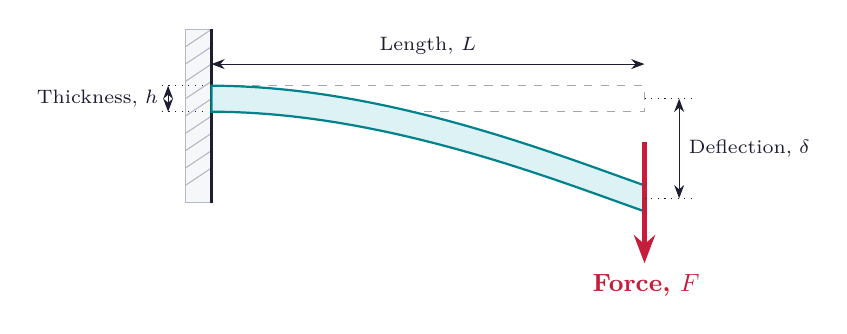
\begin{tikzpicture}[x=1.1cm, y=1.1cm, >=Stealth]
  % Clamped wall
  \draw[fill=mygray, draw=mgframe] (-0.3,-1.2) rectangle (0,0.8);
  \foreach \y in {-1.0,-0.8,...,0.6} {
    \draw[mgframe, thin] (-0.3,\y) -- (0,\y+0.2);
  }
  \draw[mydark, thick] (0,-1.2) -- (0,0.8);
  
  % Undeflected Beam
  \draw[mydark, dashed, opacity=0.4] (0,-0.15) rectangle (5.0,0.15);
  \draw[<->, mydark, thin] (0, 0.4) -- (5.0, 0.4) node[midway, above, font=\scriptsize] {Length, $L$};
  
  % Deflected Beam
  \draw[fill=hdrteal, draw=myteal, thick] 
    (0, 0.15) .. controls (2.0, 0.15) and (4.0, -0.65) .. (5.0, -1.0) -- 
    (5.0, -1.3) .. controls (4.0, -0.95) and (2.0, -0.15) .. (0, -0.15) -- cycle;
     
  % Force arrow
  \draw[redarrow, ultra thick] (5.0, -0.5) -- (5.0, -1.9) node[below, font=\small\bfseries\color{myred}] {Force, $F$};
  
  % Deflection dimension
  \draw[<->, mydark, thin] (5.4, 0) -- (5.4, -1.15) node[midway, right, font=\scriptsize] {Deflection, $\delta$};
  \draw[mydark, dotted] (5.0, 0) -- (5.6, 0);
  \draw[mydark, dotted] (5.0, -1.15) -- (5.6, -1.15);
  
  % Label thickness
  \draw[<->, mydark, thin] (-0.5, -0.15) -- (-0.5, 0.15) node[midway, left, font=\scriptsize] {Thickness, $h$};
  \draw[mydark, dotted] (-0.1, -0.15) -- (-0.6, -0.15);
  \draw[mydark, dotted] (-0.1, 0.15) -- (-0.6, 0.15);
\end{tikzpicture}
\end{tcolorbox}

The bending moment at any position $x$ along the beam length is:
$$M(x) = -F(L-x)$$
According to Euler-Bernoulli beam theory:
$$E I \frac{d^2 y}{dx^2} = M(x) = -F(L-x)$$
where $I$ is the rectangular moment of inertia:
$$I = \frac{w h^3}{12}$$
Integrate the differential equation once with respect to $x$:
$$E I \frac{dy}{dx} = -F \left(L x - \frac{x^2}{2}\right) + C_1$$
Applying the boundary condition at the clamped end ($x = 0$): $\frac{dy}{dx} = 0 \implies C_1 = 0$.
Integrate a second time:
$$E I y(x) = -F \left(L \frac{x^2}{2} - \frac{x^3}{6}\right) + C_2$$
Applying the boundary condition at $x = 0$: $y(0) = 0 \implies C_2 = 0$.
Thus, the deflection curve of the beam is:
$$y(x) = -\frac{F}{6 E I} (3 L x^2 - x^3)$$
The maximum deflection $\delta$ occurs at the free end $x = L$:
$$\delta = |y(L)| = \frac{F L^3}{3 E I}$$
Using the spring relation $F = k \delta$, the equivalent spring constant $k$ is:
$$k = \frac{3 E I}{L^3}$$
Substituting $I = \frac{w h^3}{12}$:
$$k = \frac{3 E}{L^3} \left(\frac{w h^3}{12}\right) = \frac{E w h^3}{4 L^3}$$

% ===============================================================================
\section{Coupled Electromechanical Pull-in Model}
% ===============================================================================

An electrostatic parallel-plate actuator experiences pull-in instability, where electrostatic forces overwhelm mechanical spring restoring forces.

\begin{tcolorbox}[tikzbox, title={Parallel-Plate Spring-Actuator Model}]
\centering
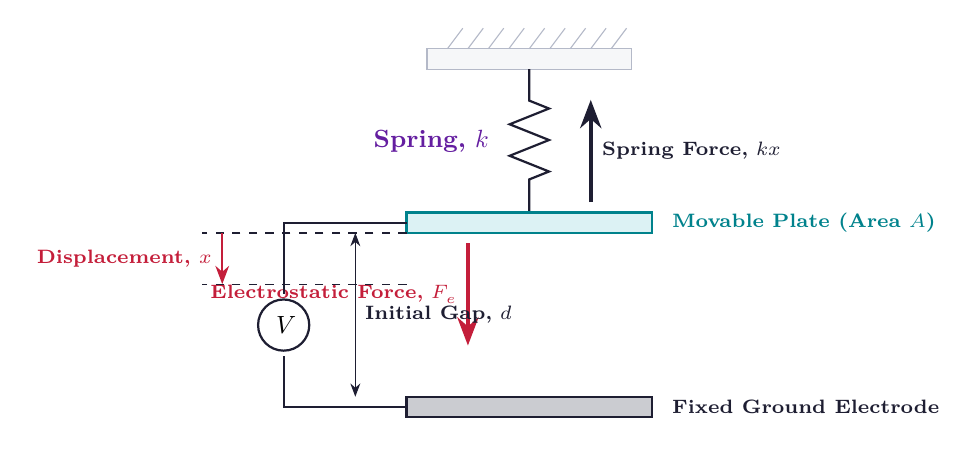
\begin{tikzpicture}[x=1.3cm, y=1.3cm, >=Stealth]
  % Rigid ceiling
  \draw[fill=mygray, draw=mgframe] (1.0,3.6) rectangle (3.0,3.8);
  \foreach \x in {1.2,1.4,...,2.8} {
    \draw[mgframe, thin] (\x,3.8) -- (\x+0.15,4.0);
  }
  
  % Spring
  \draw[mydark, thick, decoration={zigzag, pre length=4mm, post length=4mm, segment length=4mm, amplitude=2.5mm}, decorate] (2.0,3.6) -- (2.0,2.2);
  \node[anchor=east, font=\small\bfseries\color{mypurple}] at (1.7, 2.9) {Spring, $k$};
  
  % Spring Force Arrow
  \draw[arrow, ultra thick] (2.6, 2.3) -- (2.6, 3.3) node[midway, right, font=\scriptsize\bfseries\color{mygreen}] {Spring Force, $kx$};
  
  % Movable Plate
  \draw[fill=hdrteal, draw=myteal, thick] (0.8,2.0) rectangle (3.2,2.2);
  \node[anchor=west, font=\scriptsize\bfseries\color{myteal}] at (3.3,2.1) {Movable Plate (Area $A$)};
  
  % Fixed Ground Electrode
  \draw[fill=mygray!80!mydark, draw=mydark, thick] (0.8,0.2) rectangle (3.2,0.4);
  \node[anchor=west, font=\scriptsize\bfseries\color{mydark}] at (3.3,0.3) {Fixed Ground Electrode};
  
  % Electrostatic Force Arrow
  \draw[redarrow, ultra thick] (1.4, 1.9) -- (1.4, 0.9) node[midway, left, font=\scriptsize\bfseries\color{myred}] {Electrostatic Force, $F_e$};
  
  % Initial Gap Dimension Line
  \draw[<->, mydark, thin] (0.3, 0.4) -- (0.3, 2.0) node[midway, right, font=\scriptsize\bfseries] {Initial Gap, $d$};
  
  % Displacement Dashed Lines and Arrow
  \draw[dashed, mydark, thin] (0.8, 2.0) -- (-1.2, 2.0);
  \draw[dashed, mydark, thin] (0.8, 1.5) -- (-1.2, 1.5);
  \draw[->, myred, thick] (-1.0, 2.0) -- (-1.0, 1.5) node[midway, left, font=\scriptsize\bfseries] {Displacement, $x$};
  
  % Voltage source connection
  \draw[thick, mydark] (0.8,2.1) -- (-0.4,2.1) -- (-0.4,1.4);
  \draw[thick, mydark] (0.8,0.3) -- (-0.4,0.3) -- (-0.4,0.8);
  \draw[fill=white, draw=mydark, thick] (-0.4,1.1) circle (0.25);
  \node[font=\small\bfseries] at (-0.4,1.1) {$V$};
\end{tikzpicture}
\end{tcolorbox}

The force balance equation of the system at equilibrium is:
$$F_s = F_e \implies k x = \frac{1}{2} \frac{\epsilon A V^2}{(d-x)^2}$$
where $k$ is spring constant, $d$ is initial gap, and $x$ is displacement. Solve for $V^2$:
$$V^2 = \frac{2 k x (d-x)^2}{\epsilon A}$$
To find the limits of stable equilibrium, we find the maximum voltage that can be applied by taking the derivative with respect to $x$ and setting it to zero:
$$\frac{d(V^2)}{dx} = 0 \implies \frac{2k}{\epsilon A} \frac{d}{dx} \left[ x (d-x)^2 \right] = 0$$
$$\frac{d}{dx} \left( x d^2 - 2d x^2 + x^3 \right) = d^2 - 4d x + 3x^2 = 0$$
$$(d - 3x)(d - x) = 0$$
This yields two solutions: $x = d$ (unstable limit where gap is zero) and:
$$x_{\text{pi}} = \frac{d}{3}$$

\textbf{Conclusion 1:} The critical displacement at the pull-in point is exactly one-third of the initial gap.
Substitute $x_{\text{pi}} = d/3$ back into the voltage equation to find the critical \textbf{Pull-in Voltage} ($V_{\text{pi}}$):
$$V_{\text{pi}}^2 = \frac{2 k \left(\frac{d}{3}\right) \left(d - \frac{d}{3}\right)^2}{\epsilon A} = \frac{2 k \left(\frac{d}{3}\right) \left(\frac{2d}{3}\right)^2}{\epsilon A} = \frac{8 k d^3}{27 \epsilon A}$$
$$V_{\text{pi}} = \sqrt{\frac{8 k d^3}{27 \epsilon A}}$$

% ===============================================================================
\section{Finite Element Method (FEM) Overview}
% ===============================================================================

Analytical models are insufficient for complex structures. The Finite Element Method (FEM) provides numerical solutions by dividing a continuous model into finite sub-regions.
\begin{itemize}[leftmargin=*, itemsep=3.5pt]
  \item \textbf{Discretization (Meshing):} Subdividing the structure into discrete shapes (elements) connected at node points.
  \item \textbf{Governing Equations:} Formulation of algebraic equations for each element based on differential equations (e.g., Navier-Cauchy equations for elasticity).
  \item \textbf{Coupled-Field Analysis:} Crucial for MEMS, it simulates interactions across multiple physical domains concurrently (e.g., electrostatic field solving updates structural deflection, which in turn alters the electrostatic mesh).
\end{itemize}

\newpage
% ===============================================================================
% MANDATORY QUICK REVISION PAGE
% ===============================================================================
\begin{center}
  {\large\bfseries\color{myred} Quick Revision --- Module IV}\\[3pt]
  {\small\color{mydark} Bulk Micromachining \& Mechanics $|$ PE-EC603A}
\end{center}
\noindent{\color{myred}\rule{\linewidth}{1.2pt}}
\vspace{4pt}

\begin{tcolorbox}[formulabox, title={\textbf{Key Mechanical \& Electrostatic Equations}}]
\renewcommand{\arraystretch}{1.3}
\begin{tabularx}{\linewidth}{B{3.8cm} Y Y}
\textbf{Parameter} & \textbf{Core Equation} & \textbf{Key Variable Definition} \\
\hline
Hooke's Law (1D) & $\sigma = E \epsilon$ & Relates mechanical stress and strain \\[4pt]
Poisson's Ratio & $\nu = -\epsilon_{\text{trans}} / \epsilon_{\text{axial}}$ & Ratio of transverse to axial strain \\[4pt]
Thermal Stress & $\sigma_{\text{th}} = -E \alpha \Delta T$ & $E$: Young Modulus; $\alpha$: CTE; $\Delta T$: Temp difference \\[4pt]
Rect. Inertia & $I = w h^3 / 12$ & $w$: width; $h$: thickness of beam \\[4pt]
Cantilever Spring Const. & $k = 3EI / L^3 = E w h^3 / 4L^3$ & $L$: Beam length; $I$: Moment of Inertia \\[4pt]
Pull-in Voltage & $\displaystyle V_{\text{pi}} = \sqrt{\frac{8 k d^3}{27 \epsilon A}}$ & $k$: Spring constant; $d$: gap; $A$: Plate area \\[6pt]
Pull-in Displacement & $x_{\text{pi}} = d / 3$ & Deflection limit before electro-snapdown \\
\end{tabularx}
\end{tcolorbox}

\begin{tcolorbox}[defbox, title={\textbf{One-Line Definitions}}]
\begin{itemize}[leftmargin=*, itemsep=2.5pt, topsep=0pt]
  \item \textbf{Bulk Micromachining:} A fabrication technique where substrate material is removed to define micro-structures.
  \item \textbf{HNA:} An isotropic silicon wet etchant consisting of Hydrofluoric acid, Nitric acid, and Acetic acid.
  \item \textbf{Anisotropic Etch:} A directional etch that exhibits different rates along different crystallographic planes (e.g., KOH).
  \item \textbf{Anodic Bonding:} A bonding method joining silicon to sodium-rich glass using heat ($400^{\circ}\text{C}$) and high voltage.
  \item \textbf{Eutectic Bonding:} A bonding process using a gold-silicon interface heated to $363^{\circ}\text{C}$ to form a liquid-alloy bond.
  \item \textbf{Hooke's Law:} Linear relationship between stress and strain within the elastic limit of a material.
  \item \textbf{Young's Modulus ($E$):} A measure of the elastic stiffness of a solid material; equal to stress divided by strain.
  \item \textbf{Pull-in Instability:} The electrostatic collapse of a suspended electrode when displacement exceeds one-third of the gap.
  \item \textbf{FEM:} A numerical modeling technique that solves complex engineering physics problems by discretization (meshing).
\end{itemize}
\end{tcolorbox}

\begin{tcolorbox}[exambox, title={\textbf{Frequently Asked / Viva Questions}}]
\begin{enumerate}[topsep=0pt, label=\textbf{Q\arabic*.}, itemsep=5pt]
  \item \Q{Why does KOH etch the $\{111\}$ plane of Silicon much slower than the $\{100\}$ plane?}
    Because the $\{111\}$ plane has the highest atomic packing density, and surface atoms on $\{111\}$ expose only a single dangling bond (compared to two on $\{100\}$), making it chemically highly stable.
  \item \Q{Calculate the sidewall slope angle of a KOH-etched pyramidal cavity on $\{100\}$ silicon.}
    The angle between the $\{100\}$ plane and the $\{111\}$ plane is exactly $54.74^{\circ}$.
  \item \Q{Compare direct bonding and anodic bonding in MEMS packaging.}
    Direct bonding links silicon-to-silicon at high temperatures ($>1000^{\circ}\text{C}$). Anodic bonding links silicon-to-glass at lower temperatures ($300-450^{\circ}\text{C}$) using a high electrostatic field.
  \item \Q{Explain the physical meaning of Poisson's ratio ($\nu$).}
    It is the ratio of lateral contraction strain to longitudinal extension strain under tensile stress. For silicon, $\nu \approx 0.28$.
  \item \Q{State Hooke's Law and its generalized formulation in 3D for isotropic materials.}
    Hooke's Law states that stress is directly proportional to strain: $\sigma = E \epsilon$. In 3D, taking into account transverse Poisson contraction, the strains are: $\epsilon_x = \frac{1}{E} [\sigma_x - \nu(\sigma_y + \sigma_z)]$ (symmetrically for $\epsilon_y$ and $\epsilon_z$).
  \item \Q{How is thermal stress generated in clamped micro-structures?}
    If a micro-beam is anchored at both ends, thermal expansion is restricted. Heating by $\Delta T$ induces compressive thermal stress $\sigma_{\text{th}} = -E \alpha \Delta T$.
  \item \Q{State the spring constant equation of a rectangular cantilever beam and its dependency on parameters.}
    $k = \frac{E w h^3}{4 L^3}$. It is directly proportional to width ($w$) and the cube of thickness ($h^3$), and inversely proportional to the cube of length ($L^3$).
  \item \Q{Derive why pull-in displacement occurs at exactly one-third of the initial gap ($d/3$).}
    By setting the derivative of voltage squared $\frac{d(V^2)}{dx} = 0$ for the force-balance equation $k x = \frac{\epsilon A V^2}{2(d-x)^2}$, we obtain the equation $d^2 - 4dx + 3x^2 = 0$, which factorizes to yield $x_{\text{pi}} = d/3$.
  \item \Q{What happens to an electrostatic parallel-plate actuator when the voltage exceeds $V_{\text{pi}}$?}
    The electrostatic force increases faster than the spring restoring force, causing the movable plate to collapse and snap down onto the fixed electrode (pull-in).
  \item \Q{Why is coupled-field analysis necessary in FEM simulation of MEMS?}
    Because MEMS involves coupled physics (e.g. electromechanical). Electrostatic fields deform structures, which changes the electrostatic gap, altering the field. The solver must iteratively couple both solvers.
  \item \Q{Detail the chemical mechanism of isotropic silicon etching in HNA.}
    Nitric acid ($HNO_3$) oxidizes Silicon to form $SiO_2$, Hydrofluoric acid ($HF$) dissolves the $SiO_2$, and Acetic acid ($CH_3COOH$) dilutes and buffers the reaction.
\end{enumerate}
\tcbset{breakable}
\end{tcolorbox}


\end{document}
